%%%%%%%%%%%%%%%%%%%%%%%%%%%%%%%%%%%%%%%%%
% Masters/Doctoral Thesis 
% LaTeX Template
% Version 2.2 (21/11/15)
%
% This template has been downloaded from:
% http://www.LaTeXTemplates.com
%
% Version 2.x major modifications by:
% Vel (vel@latextemplates.com)
%
% This template is based on a template by:
% Steve Gunn (http://users.ecs.soton.ac.uk/srg/softwaretools/document/templates/)
% Sunil Patel (http://www.sunilpatel.co.uk/thesis-template/)
%
% Template license:
% CC BY-NC-SA 3.0 (http://creativecommons.org/licenses/by-nc-sa/3.0/)
%
%%%%%%%%%%%%%%%%%%%%%%%%%%%%%%%%%%%%%%%%%

%----------------------------------------------------------------------------------------
%	PACKAGES AND OTHER DOCUMENT CONFIGURATIONS
%----------------------------------------------------------------------------------------

\documentclass[
11pt, % The default document font size, options: 10pt, 11pt, 12pt
oneside, % Two side (alternating margins) for binding by default, uncomment to switch to one side
english, % ngerman for German
singlespacing, % Single line spacing, alternatives: onehalfspacing or doublespacing
%draft, % Uncomment to enable draft mode (no pictures, no links, overfull hboxes indicated)
%nolistspacing, % If the document is onehalfspacing or doublespacing, uncomment this to set spacing in lists to single
%liststotoc, % Uncomment to add the list of figures/tables/etc to the table of contents
%toctotoc, % Uncomment to add the main table of contents to the table of contents
%parskip, % Uncomment to add space between paragraphs
%nohyperref, % Uncomment to not load the hyperref package
headsepline, % Uncomment to get a line under the header
]{MastersDoctoralThesis} % The class file specifying the document structure

\usepackage[utf8]{inputenc} % Required for inputting international characters
\usepackage[T1]{fontenc} % Output font encoding for international characters
\usepackage{csquotes}
\usepackage{palatino} % Use the Palatino font by default

\usepackage{datetime}
\usepackage{pgfplots}

\usepackage{amsmath}
\usepackage{float}
\usepackage{listings}

\newdateformat{monthyeardate}{%
  \monthname[\THEMONTH], \THEYEAR} % Set the date format
  
  % Define some commands to keep the formatting separated from the content 
\newcommand{\keyword}[1]{\textbf{#1}}
\newcommand{\tabhead}[1]{\textbf{#1}}
\newcommand{\code}[1]{\texttt{#1}}
\newcommand{\file}[1]{\texttt{\bfseries#1}}
\newcommand{\option}[1]{\texttt{\itshape#1}}

% Suppress underfull hbox
\hbadness = 10000
% Supress overfull hbox
\hfuzz=\maxdimen

%----------------------------------------------------------------------------------------
% SETTINGS TO REMOVE ALL FIGURES
%----------------------------------------------------------------------------------------

%\usepackage{comment}
%\excludecomment{figure}
%\let\endfigure\relax

%----------------------------------------------------------------------------------------
%	BIBTEX SETTINGS
%----------------------------------------------------------------------------------------

\usepackage[backend=bibtex,bibstyle=ieee, citestyle=numeric-comp,natbib=true]{biblatex} % User the bibtex backend with the authoryear citation style (which resembles APA)
\pgfplotsset{compat=1.12}

\addbibresource{references.bib} % The filename of the bibliography


%----------------------------------------------------------------------------------------
%	TODO SETTINGS
%----------------------------------------------------------------------------------------

\usepackage{xargs}
\usepackage[colorinlistoftodos,prependcaption,textsize=tiny]{todonotes}
\newcommandx{\unsure}[2][1=]{\todo[linecolor=red,backgroundcolor=red!25,bordercolor=red,#1]{#2}}
\newcommandx{\change}[2][1=]{\todo[linecolor=blue,backgroundcolor=blue!25,bordercolor=blue,#1]{#2}}
\newcommandx{\alert}[2][1=]{\todo[linecolor=yellow,backgroundcolor=yellow!25,bordercolor=yellow,#1]{#2}}
\newcommandx{\writeSec}[2][1=]{\todo[linecolor=YellowOrange,backgroundcolor=YellowOrange!25,bordercolor=YellowOrange,#1]{#2}}
\newcommandx{\info}[2][1=]{\todo[linecolor=OliveGreen,backgroundcolor=OliveGreen!25,bordercolor=OliveGreen,#1]{#2}}
\newcommandx{\improvement}[2][1=]{\todo[linecolor=Plum,backgroundcolor=Plum!25,bordercolor=Plum,#1]{#2}}
\newcommandx{\thiswillnotshow}[2][1=]{\todo[disable,#1]{#2}}


%----------------------------------------------------------------------------------------
%	MARGIN SETTINGS
%----------------------------------------------------------------------------------------

\geometry{
	paper=a4paper, % Change to letterpaper for US letter
	inner=2.5cm, % Inner margin 2.5
	outer=3.8cm, % Outer margin
	bindingoffset=2cm, % Binding offset
	top=1.5cm, % Top margin
	bottom=1.5cm, % Bottom margin
	%showframe,% show how the type block is set on the page
}

%----------------------------------------------------------------------------------------
%	PYTHON SYNTAX HIGHLIGHTING
%----------------------------------------------------------------------------------------

% Default fixed font does not support bold face
\DeclareFixedFont{\ttb}{T1}{txtt}{bx}{n}{12} % for bold
\DeclareFixedFont{\ttm}{T1}{txtt}{m}{n}{12}  % for normal

% Custom colors
\usepackage{color}
\definecolor{deepblue}{rgb}{0,0,0.5}
\definecolor{deepred}{rgb}{0.6,0,0}
\definecolor{deepgreen}{rgb}{0,0.5,0}

% Python style for highlighting
\newcommand\pythonstyle{\lstset{
language=Python,
basicstyle=\ttm,
otherkeywords={self},             % Add keywords here
keywordstyle=\ttb\color{deepblue},
emph={MyClass,__init__},          % Custom highlighting
emphstyle=\ttb\color{deepred},    % Custom highlighting style
stringstyle=\color{deepgreen},
frame=tb,                         % Any extra options here
showstringspaces=false            % 
}}

% Python environment
\lstnewenvironment{python}[1][]
{
\pythonstyle
\lstset{#1}
}
{}

% Python for external files
\newcommand\pythonexternal[2][]{{
\pythonstyle
\lstinputlisting[#1]{#2}}}

% Python for inline
\newcommand\pythoninline[1]{{\pythonstyle\lstinline!#1!}}

%----------------------------------------------------------------------------------------
%	JSON SYNTAX HIGHLIGHTING
%----------------------------------------------------------------------------------------

\colorlet{punct}{red!60!black}
\definecolor{background}{HTML}{EEEEEE}
\definecolor{delim}{RGB}{20,105,176}
\colorlet{numb}{magenta!60!black}

\lstdefinelanguage{json}{
    basicstyle=\normalfont\ttfamily,
    numbers=left,
    numberstyle=\scriptsize,
    stepnumber=1,
    numbersep=8pt,
    showstringspaces=false,
    breaklines=true,
    frame=lines,
    backgroundcolor=\color{background},
    literate=
     *{0}{{{\color{numb}0}}}{1}
      {1}{{{\color{numb}1}}}{1}
      {2}{{{\color{numb}2}}}{1}
      {3}{{{\color{numb}3}}}{1}
      {4}{{{\color{numb}4}}}{1}
      {5}{{{\color{numb}5}}}{1}
      {6}{{{\color{numb}6}}}{1}
      {7}{{{\color{numb}7}}}{1}
      {8}{{{\color{numb}8}}}{1}
      {9}{{{\color{numb}9}}}{1}
      {:}{{{\color{punct}{:}}}}{1}
      {,}{{{\color{punct}{,}}}}{1}
      {\{}{{{\color{delim}{\{}}}}{1}
      {\}}{{{\color{delim}{\}}}}}{1}
      {[}{{{\color{delim}{[}}}}{1}
      {]}{{{\color{delim}{]}}}}{1},
}

           
%----------------------------------------------------------------------------------------
%	THESIS INFORMATION
%----------------------------------------------------------------------------------------

\thesistitle{Machine learning techniques for flow-based network intrusion detection systems} % Your thesis title, this is used in the title and abstract, print it elsewhere with \ttitle
\advisor{Prof. Dr. Peter \textsc{Quax} \\ Prof. Dr. Wim \textsc{Lamotte} \\}  % Your supervisor's name, this is used in the title page, print it elsewhere with \supname
\supervisor{Bram \textsc{Bonne} \\ Pieter \textsc{Robyns}} % Your supervisor's name, this is used in the title page, print it elsewhere with \supname
\examiner{} % Your examiner's name, this is not currently used anywhere in the template, print it elsewhere with \examname
\degree{Bachelor of Science} % Your degree name, this is used in the title page and abstract, print it elsewhere with \degreename
\author{Axel \textsc{Faes}} % Your name, this is used in the title page and abstract, print it elsewhere with \authorname
\addresses{} % Your address, this is not currently used anywhere in the template, print it elsewhere with \addressname

\subject{Computer Science} % Your subject area, this is not currently used anywhere in the template, print it elsewhere with \subjectname
\keywords{} % Keywords for your thesis, this is not currently used anywhere in the template, print it elsewhere with \keywordnames
\university{\href{http://www.uhasselt.be}{University of Hasselt}} % Your university's name and URL, this is used in the title page and abstract, print it elsewhere with \univname
\department{{Computer Science}} % Your department's name and URL, this is used in the title page and abstract, print it elsewhere with \deptname
\faculty{{Wetenschappen}} % Your faculty's name and URL, this is used in the title page and abstract, print it elsewhere with \facname
\group{{Networks and Security}}

\hypersetup{pdftitle=\ttitle} % Set the PDF's title to your title
\hypersetup{pdfauthor=\authorname} % Set the PDF's author to your name
\hypersetup{pdfkeywords=\keywordnames} % Set the PDF's keywords to your keywords

\renewcommand{\cleardoublepage}{\clearpage}

%----------------------------------------------------------------------------------------
%	BEGIN DOCUMENT
%----------------------------------------------------------------------------------------

\begin{document}

\frontmatter % Use roman page numbering style (i, ii, iii, iv...) for the pre-content pages

\pagestyle{plain} % Default to the plain heading style until the thesis style is called for the body content

%----------------------------------------------------------------------------------------
%	TITLE PAGE
%----------------------------------------------------------------------------------------

\begin{titlepage}
\begin{center}

\textsc{\LARGE \univname}\\[1.5cm] % University name

\textsc{\Large Bachelor Thesis}\\[0.5cm] % Thesis type

\HRule \\[0.4cm] % Horizontal line
{\huge \bfseries \ttitle}\\[0.4cm] % Thesis title
\HRule \\[1.5cm] % Horizontal line
 
\begin{minipage}{0.4\textwidth}
\begin{flushleft} \large
\emph{Author:}\\
{\authorname} % Author name - remove the \href bracket to remove the link
\end{flushleft}
\end{minipage}
\begin{minipage}{0.4\textwidth}
\begin{flushright} \large
\emph{Advisor:} \\
{\adname} % Supervisor name - remove the \href bracket to remove the link 

\emph{Mentor:} \\
{\supname} % Supervisor name - remove the \href bracket to remove the link 
\end{flushright}
\end{minipage}\\[1.5cm]
 
\large \textit{Bachelorproef voorgedragen tot het behalen van de graad van bachelor in de informatica/ICT/kennistechnologie}\\[0.3cm]
\large \textit{A thesis submitted in fulfillment of the requirements\\ for the degree of \degreename}\\[0.3cm] % University requirement text
\textit{in the}\\[0.4cm]
\groupname\\\deptname\\[1cm] % Research group name and department name
 
{\large Academiejaar 2015-2016}~\\
{\large \monthyeardate\today}~\\[1cm] % Date
%\includegraphics{Logo} % University/department logo - uncomment to place it
 
\includegraphics[width=0.7\textwidth]{LOGO}~\\[1cm]

\vfill
\end{center}
\end{titlepage}

%\begin{titlepage}
%\begin{center}
%
%\textsc{\LARGE \univname}\\[1cm] % University name
%
%\textsc{\Large Bachelor Thesis}\\[0.5cm] % Thesis type
%
%\HRule \\[0.4cm] % Horizontal line
%{\huge \bfseries \ttitle}\\[0.4cm] % Thesis title
%\HRule \\[0.5cm] % Horizontal line
% 
%\begin{minipage}{0.4\textwidth}
%\begin{flushleft} \large
%\emph{Author:}\\
%{\authorname} % Author name - remove the \href bracket to remove the link
%\end{flushleft}
%\end{minipage}
%\begin{minipage}{0.4\textwidth}
%\begin{flushright} \large
%\emph{Supervisor:} \\
%{\supname} % Supervisor name - remove the \href bracket to remove the link  
%\end{flushright}
%\end{minipage}\\[1cm]
% 
%\large \textit{Bachelorproef voorgedragen tot het behalen van de graad van bachelor in de informatica/ICT/kennistechnologie}\\[0.3cm]
%\large \textit{A thesis submitted in fulfillment of the requirements\\ for the degree of \degreename}\\[0.3cm] % University requirement text
%\textit{in the}\\[0.4cm]
%\groupname\\\deptname\\[0.5cm] % Research group name and department name
% 
%{\large \monthyeardate\today}~\\[0.5cm] % Date
%%\includegraphics{Logo} % University/department logo - uncomment to place it
% 
\includegraphics[width=0.7\textwidth]{LOGO}~\\[0.5cm]
%
%\vfill
%\end{center}
%\end{titlepage}

%----------------------------------------------------------------------------------------
%	DECLARATION PAGE
%----------------------------------------------------------------------------------------

\begin{declaration}
\addchaptertocentry{\authorshipname}

\noindent I, \authorname, declare that this thesis titled, \enquote{\ttitle} and the work presented in it are my own. I confirm that:

\begin{itemize} 
\item This work was done wholly or mainly while in candidature for a bachelor degree at this University.
\item Where any part of this thesis has previously been submitted for a degree or any other qualification at this University or any other institution, this has been clearly stated.
\item Where I have consulted the published work of others, this is always clearly attributed.
\item Where I have quoted from the work of others, the source is always given. With the exception of such quotations, this thesis is entirely my own work.
\item I have acknowledged all main sources of help.
\item Where the thesis is based on work done by myself jointly with others, I have made clear exactly what was done by others and what I have contributed myself.\\
\end{itemize}
 
\noindent Signed:\\
\rule[0.5em]{25em}{0.5pt} % This prints a line for the signature
 
\noindent Date:\\
\rule[0.5em]{25em}{0.5pt} % This prints a line to write the date
\end{declaration}

%----------------------------------------------------------------------------------------
%	ABSTRACT PAGE
%----------------------------------------------------------------------------------------

\begin{abstract}
\addchaptertocentry{\abstractname} % Add the abstract to the table of contents

\noindent Large data centers are storing and sending more and more data. In order to check whether the network traffic does not contain intrusions, an intrusion detection system is used. Such a system analyses data from the network and gives an alert if it finds an intrusion. Since data centers have so much data traffic, it is difficult to process everything. That's where IP flows come in the picture. They are aggregated from packet data but do not contain any information about the payload data. This thesis explains which attacks can be detected and how IP flows can be used for intrusion detection. It would also be cost-efficient if an intrusion detection system could operate automatically and detect attacks with a high probability. For this machine learning can be used. Machine learning is a type of Artificial Intelligence which allows programs to learn and find patterns within data. However, there are many different types of machine learning. This thesis gives an introduction to machine learning concepts and gives an overview of different machine learning algorithms such as Support Vector Machines and K-Nearest Neighbors. An explanation is given on how these algorithms can be used in an intrusion detection system. The algorithms are evaluated on different datasets which consist of both labeled training data and unlabeled real world data. In the evaluation it is found that supervised learning gives better and more detailed predictions as compared to unsupervised learning. K-Nearest Neighbors gives the best results among the tested supervised learning algorithms. The results show that machine learning is a viable option to detect intrusions using IP flows. 

\end{abstract}

%----------------------------------------------------------------------------------------
%	ACKNOWLEDGEMENTS
%----------------------------------------------------------------------------------------

\begin{acknowledgements}
\addchaptertocentry{\acknowledgementname} % Add the acknowledgements to the table of contents

%The acknowledgments and the people to thank go here, don't forget to include your project advisor\ldots
\noindent I would like to thank my mentor, Bram Bonne, with whom I had weekly meetings. He has given feedback on this thesis and had a lot of suggestions regarding the machine learning chapters. I would like to thank Cegeka, to provide me with a dataset on which I could test the implementation. Thanks also go towards my promotor professor Peter Quax and co-promotor professor Wim Lamotte for their advise and providing me with the EDM dataset. \\
\\
From my classmates, I would like to thank Matthijs Kaminski for his support throughout the bachelor. I would also like to thank Luuk Raaijmakers for reading over my thesis.

\end{acknowledgements}

%----------------------------------------------------------------------------------------
%	LIST OF CONTENTS/FIGURES/TABLES PAGES
%----------------------------------------------------------------------------------------

\setcounter{tocdepth}{1}
\tableofcontents % Prints the main table of contents

\listoffigures % Prints the list of figures

\listoftables % Prints the list of tables

%----------------------------------------------------------------------------------------
%	ABBREVIATIONS
%----------------------------------------------------------------------------------------

\begin{abbreviations}{ll} % Include a list of abbreviations (a table of two columns)

\textbf{IDS} & \textbf{I}ntrusion \textbf{D}etection \textbf{S}ystem\\
\textbf{IPS} & \textbf{I}ntrusion \textbf{P}revention \textbf{S}ystem\\
\textbf{IDPS} & \textbf{I}ntrusion \textbf{D}etection (and) \textbf{P}revention \textbf{S}ystem\\
\textbf{NIDS} & \textbf{N}etwork (based) \textbf{I}ntrusion \textbf{D}etection \textbf{S}ystem\\
\textbf{HIDS} & \textbf{H}ost (based) \textbf{I}ntrusion \textbf{D}etection \textbf{S}ystem\\
\textbf{SIEM} & \textbf{S}ecurity \textbf{I}nformation and \textbf{E}vent \textbf{M}anagement 
\\
\textbf{DDOS} & \textbf{D}tributed \textbf{D}enial \textbf{o}f \textbf{S}ervice  \\
\\
\textbf{ML} & \textbf{M}achine \textbf{L}earning\\
\textbf{MSE} & \textbf{M}inimum \textbf{S}quared \textbf{E}rror (function)\\
\\
\textbf{KNN} & \textbf{K}-\textbf{N}erest \textbf{N}eighbors\\
\textbf{SVM} & \textbf{S}upport \textbf{V}ector \textbf{M}achines\\

\end{abbreviations}
%----------------------------------------------------------------------------------------
%	SYMBOLS
%----------------------------------------------------------------------------------------

\begin{symbols}{lll} % Include a list of Symbols (a three column table)

$H_0(x)$ & Hypothesis function \\
$J(\theta)$ & Cost function \\
%$P$ & power & \si{\watt} (\si{\joule\per\second}) \\
%Symbol & Name & Unit \\

\addlinespace % Gap to separate the Roman symbols from the Greek

%$\omega$ & angular frequency & \si{\radian} \\

\end{symbols}
%----------------------------------------------------------------------------------------
%	DEDICATION
%----------------------------------------------------------------------------------------

%\dedicatory{For/Dedicated to/To my\ldots} 

%----------------------------------------------------------------------------------------
%	THESIS CONTENT - CHAPTERS
%----------------------------------------------------------------------------------------

\mainmatter % Begin numeric (1,2,3...) page numbering

\pagestyle{thesis} % Return the page headers back to the "thesis" style

\begin{samenvatting}
\addchaptertocentry{\nederlandsesamenvatting}

\writeSec{Write the samenvatting in dutch}

\section{Intrusion detection systems}

\section{IP Flows}

\section{Machine learning}

\section{Conclusies}

\end{samenvatting}
% Chapter 1

\chapter{Introduction} % Main chapter title

\label{Chapter1} % Change X to a consecutive number; for referencing this chapter elsewhere, use \ref{ChapterX}

The internet is constantly growing and new network sevices arise constantly. This has as effect that security flaws become more and more important. Considering this, it becomes more important to be able to detect and prevent attacks on network systems.

\section{Intrusion detection systems}
An intrusion detection system is a system which tries to determine whether a system is under attack, to detect intrusions within a system. There are different types of intrusion detection systems or IDS. There are network-based intrusion detection systems and host-based intrusion detection systems. This thesis will uses machine learning techniques to detect malicious network behaviour, as such only network-based intrusion detection systems are covered.
\begin{figure}[H]
\centering
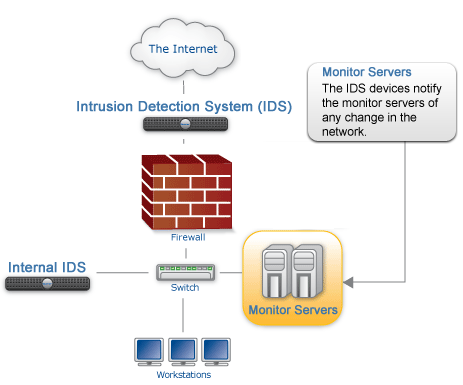
\includegraphics[width=0.6\textwidth]{Figures/idsdiagram}
\decoRule
\caption[Possible placement of IDS]{An IDS can for example be placed within the network or just before the network.}
\label{fig:IDS}
\end{figure}
\subsection{Host-based Intrusion Detection Systems}
Host-based intrusion detection systems are systems that monitor the device on which they are installed. The way they monitor the system can range from monitoring the state of the main system through log files, to monitoring program execution. In this way they can be quite indistinguishable from Anti-Virus programs.

\subsection{Network-based Intrusion Detection Systems}
Network-based intrusion detection systems are placed at certain points within a network in order to monitor traffic from and to devices within the network. The system can analyse the traffic using multiple techniques to determine whether the data is malicious. There are two different ways to analyse the network data. The analysis can be packet-based or flow-based.\\
\\
Packet-based analysis uses the entire packet including the headers and payload. An intrusion detection system that uses packet-based analysis is called a packet-based network intrusion detection system. The advantage of this type of analysis is that there is a lot of data to work with. Every single byte of the packet could be used to determine whether the packet is malicious or not. The disadvantage is immediately obvious once we look at networks through which a lot of data passes, such as data centers. Analysing every byte is very work-intensive and near impossible to do in such environments. \cite{alaidaros2011overview} \\
\\
Flow-based analysis doesn't use individual packets but uses general data about network flows. An intrusion detection system that uses flow-based analysis is called a flow-based network intrusion detection system. A flow is defined as a single connection between the host and another device. A flow can be defined using a (source\_IP, destination\_IP, source\_port, destination\_port) tuple. However flowdata also contains other information such as the duration of the connection, the start time, the amount of bytes and/or packets within the flow. Flow data can even contain data such as the amount of SYN packets within the flow. This could be useful to detect SYN overflow attacks. However not every flow collector collects this data Since flow data is much more compact than all the individual packets, it is much more feasable for data centers to use flow-based intrusion detection systems. 

\subsection{Intrusion Prevention Systems}
An intrusion prevention system or IPS/IDPS is an intrusion detection system that also has to ability to prevent attacks. An IDS does not necessarily need to be able to detect attacks at the exact moment they occur, although it is preferred. An IPS needs to be able to detect attacks real-time since it also needs to be able to prevent these attacks. For network attacks these prevention actions could be closing the connection, blocking an IP, limiting the data throughput.

\section{IP Flows}
\label{export}
Flows are aggregated from all packet data that travels through the network. Flow exporters are programs which collect network packets and aggregate them into flow records. A flow is not the same as a TCP connection. A flow can be any communication between two devices with any protocol. Flows are defined using a (source\_IP, destination\_IP, protocol) tuple. This is why flows are also called IP Flows.\\
\\
Since flow data does not contain any payload information, intrusion detection systems that use flow data cannot detect malicious behaviour embedded within payload data. \cite{IPFlow}

\section{Detection}
There are mutliple different methods to detect intrusions. There are \textbf{Signatures based methods} and there are \textbf{Anomaly Based} methods. Both of these methods have their own strengths and weaknesses. \cite{methods}
\subsection{Signature based methods}
\begin{figure}[H]
\centering
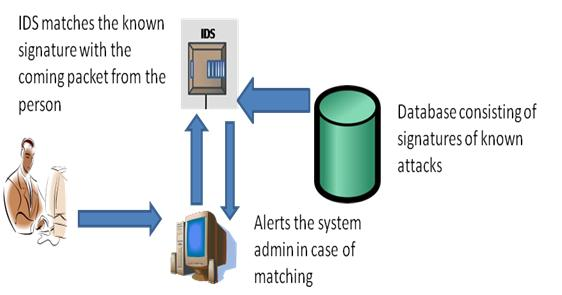
\includegraphics[width=0.7\textwidth]{Figures/Signature-based-Intrusion-Detection-System}
\decoRule
\caption[Signature based IDS]{An Signature-based intrusion detection system.}
\label{fig:Signature}
\end{figure}
\noindent Signature based methods compare so called "signatures" with an existing database of signatures. An packet or flow record is decomposed into features that together construct a signature. If the signature of an incoming flow or packet matches with a signature in the database, it is flagged as malicious. Signature-based methods have little overhead in both computation and preprocessing as it only tries to match incoming signatures to known signatures in the database. Because it only compares signatures, it is easy to deploy within a network. The system does not need to learn what the traffic within a network looks like. \\
\\
Signature based methods are very effective against known attacks. New attacks cannot be detected unless the database is updated with new signatures. It is also for attackers to avoid being caught by signature based methods, only slight modification of the "signature" is required in order to bypass the exact matching. Updating the signature database requires a lot of technical effort, since new attacks are discovered all the time.
\subsection{Anomaly based methods}
\begin{figure}[H]
\centering
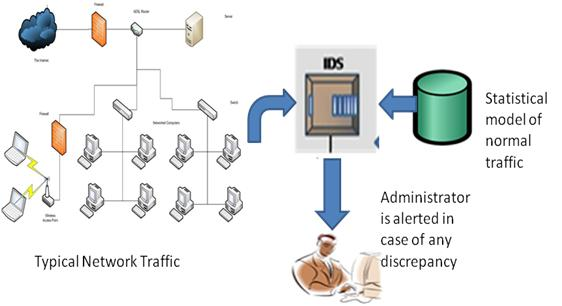
\includegraphics[width=0.7\textwidth]{Figures/Anomaly-based-Intrusion-Detection-System}
\decoRule
\caption[Anomaly based IDS]{An Anomaly-based intrusion detection system.}
\label{fig:Anomaly}
\end{figure}
\noindent Anomaly based methods, also called Behaviour based methods are methods in which the IDS tries to model the behaviour of network traffic. When an incoming packet deviates from this model, it is flagged as malicious and an alert is send. Because they use a statistical model of normal behaviour, they should be able to detect all deviations from this normal behaviour. As a result, new attacks that deviate to much from normal behaviour are detected aswell. \\
\\
Since a model of the network traffic needs to be created, the system cannot be deployed into a network and be expected to work. The system needs to learn the behaviour of the network traffic. Problems, such as generating a lot of false positive alarms, can arise when training data includes mistakes, such as misclassifications. \\
\\
Machine learning algorithms can be used as a anomaly based method. Machine learning techniques have the ability to learn from data and decide whether new data is malicous. 


\chapter{Intrusion detection systems} % Main chapter title
\label{ids}
An intrusion detection system is a system which tries to determine whether a system is under attack, to detect intrusions within a system.  Intrusion detection systems are often called IDS's. Intrusions can also be called attacks or anomalies. It does this by monitoring network or system activities. One way of categorizing IDS's is based on the method of detection intrusion. The first type would be monitoring the network, these are called network-based intrusion detection systems, or NIDS. When the intrusion detection system only monitors system activities, it is called a host-based intrusion detection system, or HIDS. \cite{sans} \\
\\
Figure~\ref{fig:IDS} shows the possible placements of an IDS. It can be placed before any firewall, being the first defense of a network. This is a NIDS. An IDS can also be placed within a network. This IDS can still monitor the network but it can also monitor system activities of the workstations. An HIDS is most commonly, but not always located on the device that it monitors.
\begin{figure}[H]
\centering
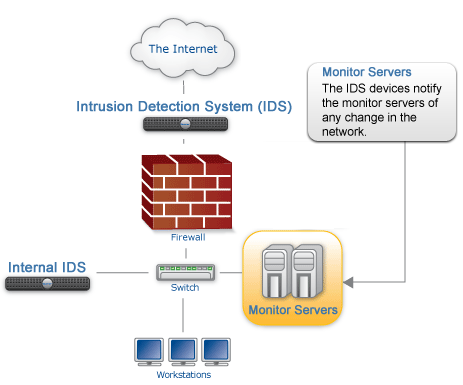
\includegraphics[width=0.9\textwidth]{Figures/idsdiagram}
\decoRule
\caption[Possible placement of IDS]{An IDS can for example be placed within the network or just before the network. \cite{ids1}}
\label{fig:IDS}
\end{figure}
\section{Host-based Intrusion Detection Systems}
Host-based intrusion detection systems are systems that monitor the device on which they are installed, or directly connected to. The way they monitor the system can range from monitoring the state of the main system through audit logs, to monitoring program execution. In this way they can be quite indistinguishable from Anti-Virus programs. \cite{sans}\\
\\
Since HIDS rely so much on audit logs, they can become limited by them. If the software that is being monitored does not provide enough information in audit logs, the IDS cannot always determine intrusions succesfully. Another issue can be the sheer volume of the audit logs. Every monitored log needs to be parsed, this means that the HIDS can have a big impact on the performance of the host system if it is installed there. \cite{Bace:1999:ID:347487} \\
\\
Another disadvantage is that any vulnerability that causes the audit files to be changed, also impacts the integrity of the HIDS. If an audit file is changed, the HIDS cannot see and detect what truly happened. \cite{Sundaram:1996:IID:332159.332161}

\section{Network-based Intrusion Detection Systems}
Network-based intrusion detection systems are placed at certain points within a network in order to monitor traffic from and to devices within the network. They operate on the same concept as wiretapping. They "tap" into a network and listen to all communication that happens.  \cite{sans} \\
\\
Using the network data instead of audit trails such as HIDS is desirable in multiple ways. One advantage is that they do not impact the performance of programs that are using the network. It is also more difficult for an intruder to attack the IDS itself. Network traffic is always visible and cannot be changed like an audit trail. The intruder could try to minimize his network activity, but the risk is lower. NIDS are also more portable than HIDS. They monitor traffic over a network and are independent of the operating system they run on.  \cite{Bace:1999:ID:347487} \\
\\
The system can analyse the traffic using multiple techniques to determine whether the data is malicious. There are two different ways to analyse the network data. The analysis can be packet-based or flow-based.\\
\\
Packet-based analysis uses the entire packet including the headers and payload. An intrusion detection system that uses packet-based analysis is called a packet-based network intrusion detection system. The advantage of this type of analysis is that there is a lot of data to work with. Every single byte of the packet could be used to determine whether the packet is malicious or not. The disadvantage is immediately obvious once we look at networks through which a lot of data passes, such as data centers. Analysing every byte is very work-intensive and near impossible to do in such environments. \cite{alaidaros2011overview} \\
\\
Flow-based analysis doesn't use individual packets but uses general aggregated data about network flows. An intrusion detection system that uses flow-based analysis is called a flow-based network intrusion detection system. A flow is defined as a single connection between the host and another device. A flow can be defined using a (source\_IP, destination\_IP, source\_port, destination\_port) tuple. However flows also contains other information. IP Flows are discussed in depth in Section~\ref{flow}. Because of the other information, flows can still contain a lot of information, even when compared to packets. Since flow data is much more compact than all the individual packets, it is much more feasable for data centers to use flow-based intrusion detection systems. \cite{alaidaros2011overview} \cite{pao2004netflow}

\subsection{Intrusion Prevention Systems}
An intrusion prevention system or IPS/IDPS is an intrusion detection system that also has to ability to prevent attacks. An IDS does not necessarily need to be able to detect attacks at the exact moment they occur, although it is preferred. An IPS needs to be able to detect attacks real-time since it also needs to be able to prevent these attacks. For network attacks these prevention actions could be closing the connection, blocking an IP or limiting the data throughput.  \cite{sans2}\\
\\
The change to requiring attacks to be detected at real time can severly impact the methods that are used to detect these attacks. For example, an IDS might give an alert even though the IDS is not certain that whatever it is alerting is actually an anomaly. An IPS needs to be certain before it can take action. Otherwise the IPS might take actions which the business employing the IPS does not want.  \cite{sans2}\\
\\
In case of a NIPS, an network-based intrusion prevention system, some advantages of being network-based are not true anymore. An NIPS needs to see all data, and preferably block network data before it reaches it's destination as seen in Figure~\ref{fig:IPS}. This means that the performance of programs using the network might be affected by the NIPS. \cite{golling2014towards}

\begin{figure}[H]
\centering
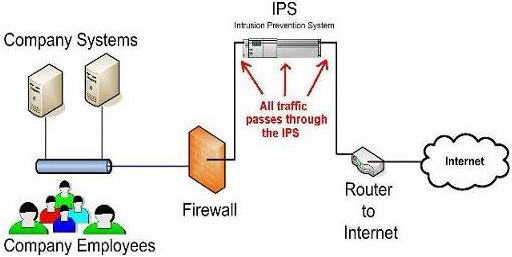
\includegraphics[width=1\textwidth]{Figures/IDS_IPS}
\decoRule
\caption[Intrusion prevention system]{An Intrusion prevention system. \cite{ips1}}
\label{fig:IPS}
\end{figure}

\section{Detection}
\label{detection}
There are mutliple different methods to detect intrusions. There are \textbf{Signature based methods} and there are \textbf{Anomaly Based} methods. Both of these methods have their own strengths and weaknesses. 
\subsection{Signature based methods}
\begin{figure}[H]
\centering
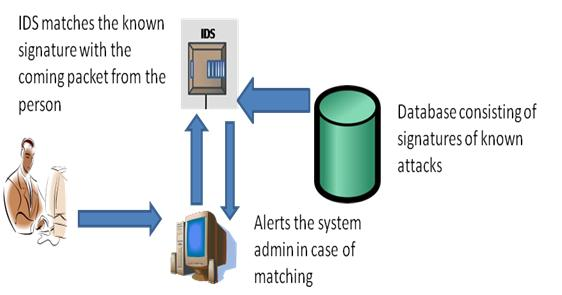
\includegraphics[width=1\textwidth]{Figures/Signature-based-Intrusion-Detection-System}
\decoRule
\caption[Signature based IDS]{An Signature-based intrusion detection system. \cite{snortImg}}
\label{fig:Signature}
\end{figure}
\noindent Signature based methods compare so called "signatures" with an existing database of signatures. An packet or flow record is decomposed into features that together construct a signature. If the signature of an incoming flow or packet matches with a signature in the database, it is flagged as malicious. Pseudocode of this can be seen below. Signature-based methods have little overhead in both computation and preprocessing as it only tries to match incoming signatures to known signatures in the database. Because it only compares signatures, it is easy to deploy within a network. The system does not need to learn what the traffic within a network looks like. \cite{methods} \\
\begin{python}
signatures = get_signatures_from_database()
while True:
    packet = get_next_packet()
    packet_signature = get_important_features(packet)
    
    if (signatures.contains(packet_signature):
        generate_alert(packet)
    else:
         # packet signature was not
         # a match with known signatures
         continue
\end{python}~\\
Signature based methods are very effective against known attacks. New attacks cannot be detected unless the database is updated with new signatures. It is also possible for attackers to avoid being caught by signature based methods, only a slight modification of the "signature" is required in order to bypass the exact matching. \cite{IPFlow}\\
\\
This could be done by trying to make the network behaviour look more like normal behaviour. For example, a botnet uses IRC communication with his master. The communication might follow certain patterns which are different from usual IRC traffic from a chat. The creator might change the botnet so that communication between the botnet and the master look similar to the usual IRC traffic. This change causes the network behaviour to be different from the signature database and not generate an alert. Updating the signature database requires a lot of technical effort, since new attacks are discovered all the time.\cite{methods} \cite{uddin2013intrusion}
\subsection{Anomaly based methods}
\begin{figure}[H]
\centering
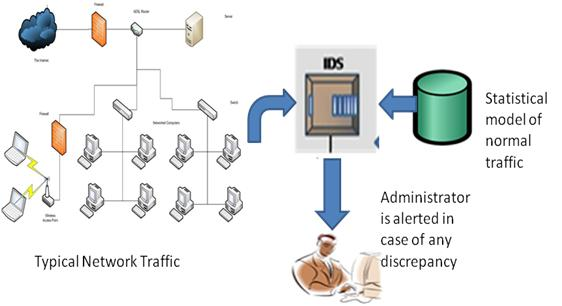
\includegraphics[width=1\textwidth]{Figures/Anomaly-based-Intrusion-Detection-System}
\decoRule
\caption[Anomaly based IDS]{An Anomaly-based intrusion detection system. \cite{snortImg}}
\label{fig:Anomaly}
\end{figure}
\noindent Anomaly based methods, also called Behaviour based methods are methods in which the IDS tries to model the behaviour of network traffic. When an incoming packet deviates from this model, it is flagged as malicious and an alert is sent. Because they use a statistical model of normal behaviour, they should be able to detect all deviations from this normal behaviour. As a result, new attacks that deviate too much from normal behaviour are detected as well. \cite{snortImg} \\
\\
Since a model of the network traffic needs to be created, the system cannot be deployed into a network and be expected to work. The system needs to learn the behaviour of the network traffic. Problems, such as generating a lot of false positive alarms, can arise when training data includes mistakes, such as misclassifications. \\
\\
Machine learning algorithms can be used as an anomaly based method. Machine learning techniques have the ability to learn from data and decide whether new data is malicous. \cite{snortImg}

\section{Existing Intrusion detection systems}
There are a lot of different intrusion detection and intrusion prevention systems on the market. Some of these systems are very expensive, others are completely open source and free. 

\subsection{Alienvault}
\textit{Alienvault} is a business that develops software to manage cyber attacks. They create SIEM solutions, Security Information and Event Management solutions. These are tools that provide methods to analyse security threats. IDS's are incorperated into SIEM's. \cite{alienvault} \\
\\
The product they make is the \textit{AlienVault Unified Security Management} (USM). USM is an all-in-one tool. USM contains a lot of tools that are required to analyse a system for cyber security threats. It contains tools that can scan and test the network for vulnerabilities. \\
\\
USM supports both host-based intrusion detection and network-based intrusion detection. It also has the option to do both full packet and netflow analysis, supporting both types of NIDS systems. \cite{alienvaultProd} \\
\\
\textit{Alienvault} works on both signature-based and anomaly-based intrusion detection. However, it is interesting to note that they are working on new strategies that can detect intrusions. Research is being done using neural networks to make intrusion detection more accurate. \cite{alienvaultIDS}

\subsection{SNORT}
Snort is an open-source network intrusion detection and prevention system. It is made to be very lightweight in use. It runs on UNIX derivatives and Windows. SNORT is the most widely used IDS worldwide and has become the in reality standard for the industry. SNORT can also operate on both packet level and IP flow level. However, SNORT uses a combination of signature and anomaly detection methods. \cite{kurundkar2012network} \\
\\
SNORT uses a system based on rules. Using rules, an administrator can configure SNORT. These rules allow for both signature and anomaly detection methods. This means that SNORT itself does not work with machine learning algorithms. However, the rules can be made using machine learning algorithms. These algorithms make rules based on which traffic is classified as normal and abnormal.  \cite{duffield2009rule} \\
\\
SNORT can, since a couple years, also be deployed as a intrusion prevention system. This is done by adding a new type of rule, a "drop" rule. A "drop" rule has higher precedence than an "alert" rule. This means that any packet that matches a "drop" rule and an "alert" rule will be dropped. \\
\\
Since SNORT is open source, the internal structure can be observed. There are several components that work together to detect abnormal behaviour and to generate output in a format that is appropriate for an intrusion detection system. \cite{kurundkar2012network}
\begin{itemize}
\item Packet sniffer and decoder
\item Preprocessors
\item Intrusion detection engine
\item Logger and alert system
\item Output modules
\end{itemize}

\noindent In Figure~\ref{fig:snort}, the structure of the SNORT components can be seen. The \textbf{packet sniffer and decoder} sniffs packets from different network interfaces. The packets are then prepared to go to the preprocessor. The \textbf{preprocessor} can already extract the most important data from packets and might even modify the data. In the \textbf{detection engine} rules are used to detect any intrusions. The rules are matched against every packet. If a packet is matched, it may be dropped or an alert can be generated, depending on the type of the rule. \\
\\
Alerts can be logged to different kinds of files. This happens in the \textbf{logger and alert system}. These could be text files or tcpdumps. The \textbf{output modules} can do different operations on the output to generate new log files.  \cite{kurundkar2012network}

\begin{figure}[H]
\centering
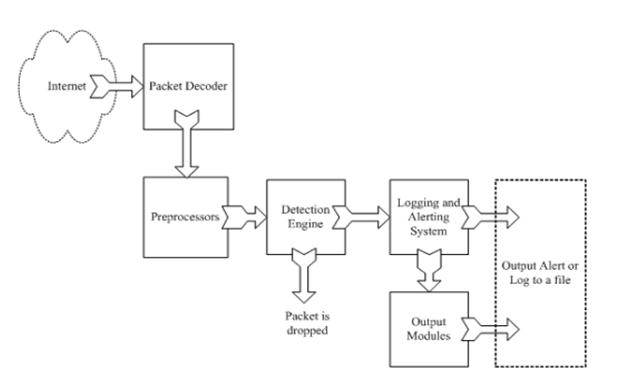
\includegraphics[width=1\textwidth]{Figures/snort}
\decoRule
\caption[The structure of the SNORT IDS]{The structure of the SNORT IDS. \cite{snortImg}}
\label{fig:snort}
\end{figure}

\subsection{MIT AI\textsuperscript{2}}
MIT is also working on methods to use machine learning to defend against cyber attacks. In their paper "\textit{AI\textsuperscript{2}: Training a big data machine to defend}", they present a new method. Their system has four components. A big data processing system, an outlier detection engine, a mechanism to obtain feedback from security analysts, and a supervised learning module.
\cite{veeramachaneniai2}\\
\\
Their system tries to combine the expertise of security experts, and the speed and ability to detect new attacks of machine learning. More specifically, they use unsupervised machine learning. They prefered to use unsupervised machine learning since labeled data is rare and attacks constantly evolve. In the system they generate their own labels and use a supervised learning algorithm with these labels. \\
\\
The \textbf{big data processing system} is a system that can extract features of different entities from raw data. The \textbf{outlier detection engine} is a system that uses unsupervised learning. It uses the features that have been found in the big data processing system. They use three different methods, density, matrix decomposition, or replicator neural networks. \cite{veeramachaneniai2} \\
\\
The output of this unsupervised system is processed and shown to a \textbf{security analyst}. The security analyst can verify or refute the output. The feedback is fed to a \textbf{supervised learning algorithm}. The supervised learning algorithm learn a model that can use this feedback to better predict whether any new event is normal or abnormal. With more feedback, the system becomes more and more correct. The flow of the system can be seen in Figure~\ref{fig:mit}. \cite{veeramachaneniai2}

\begin{figure}[H]
\centering
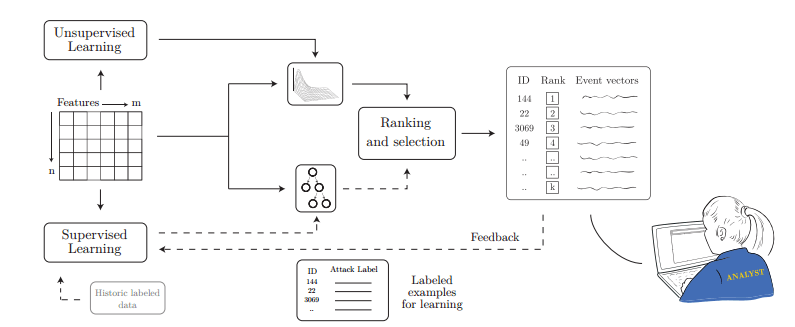
\includegraphics[width=1\textwidth]{Figures/AI2}
\decoRule
\caption[The structure of AI2 system]{The structure of AI2 system. \cite{mit2}}
\label{fig:mit}
\end{figure}

\noindent Their system has been tested by monitoring a large web-scale platform. This platform generated millions of log lines per day. The monitoring lasted three month and generated 3.6 billion log lines. They coud detect 85 percent of attacks and reduced the amount of false positives by 5 times since the previous implementation. \cite{mit2}


% Chapter 1

\chapter{Attack Classification} % Main chapter title

\label{attack} % Change X to a consecutive number; for referencing this chapter elsewhere, use \ref{ChapterX}

An intrusion detection system can use multiple methods to detect malicious behaviour. In order to make the IDS as effective as possible, the exact classifications of attacks that can be detected need to be known.

\section{Classification}
There are several types of attacks that can occur. Some of these attacks occur from within the network, other from outside the network. The exact classifications are not mutually exclusive. Some types of malware utilise network attacks. However it is important to make a distinction between these attacks. Every attack is identified by different characteristics. Knowing these characteristics is useful to be able to tweak the IDS to make identification more effective.

\section{Network attacks}
There are \textbf{Physical attacks}, these are attacks which attempt to destroy physical equipment and hardware. \textbf{Buffer overflows} are attacks that try to execute arbritrairy code or crash a process by overflowing a buffer on the targeted system. \textbf{Password attacks} attempts to break into a system by gaining the password that the system uses. The simplest password attacks are brute-force password crackers. \textbf{DDOS} attacks are attacks which attempt to make a network resource temporarily or permanently unavailable for the users of that resource. An attack could happen by flooding a system with TCP SYN packets. \textbf{Network scans} are information gathering attacks. They do not cause any damage by themselves but usually serve the purpose to gather information about a system that could be used in further attacks. Network traffic sniffing or port scans are examples of network scans. \cite{IPFlow}

\section{Malware}
There are several types of malware. There are four distinct categories of malware. There are \textbf{botnets}, \textbf{viruses}, \textbf{trojan horses} and \textbf{worms}. Malware are actual programs that infect a system to execute a specific task. The task of the malware defines which category the malware belongs in.\\
\\
\textbf{Trojan horses} are programs disguised as harmless applications but contain malicious code. \textbf{Worms} are programs that replicate themselves among a network.  They can spread extremely fast. \textbf{Viruses} are similar to worms. However they only replicate themselves on the infected host computer. Thus they require user interaction in order to be spread around a network. The virus can accomplish this by attaching itself to an email-attachment, embed itself within an executable, etc. \\
\\
\textbf{Botnets} is malware that causes infected computers to become "slaves" to the master. An infected computer is controlled externally by the bot-master without the knowledge of the owner of the infected computer. The bot-master can use the distributed network of "slave" computer to perform other malicious tasks, such as performing an DDOS attack. \cite{IPFlow}

\section{Detection}
An NIDS only monitors the network. As such not every attack can be detected by an NIDS. Only the attacks that actually use the network can be detected. Flow-based IDS have the additional constraint that they can only use flow data. This further limits the attacks that can be detected. The attacks that can be detected using a flow-based network intrusion detection systems are:
\begin{itemize}
\item DDOS
\item Network scans
\item Worms
\item Botnets
\end{itemize}
Other attacks either do not use network communication, or they are not visible within the header information of network traffic. In order to detect other attacks, including \textbf{viruses}, \textbf{trojan horses} and \textbf{Buffer overflows}, other detection systems such as HIDS or Packet-based NIDS should be used.

\subsection{Distributed Denial of Service}
A distributed denial of service can be detected by the amount of data that is being received. However, there are many different types of DDoS attacks. There are ICMP floods, SYN floods, etc. These attacks can be described in terms of traffic patterns. A traffic pattern is expressed in a couple features. These features include the number of flows and packets, the packet size, and the total bandwidth used during the traffic. For example UDP flooding can be characterised by a traffic pattern which contains a lot of packets. These patterns can be searched for during the detection phase. \cite{kim2004flow}
\subsection{Network scans}
There are three categories of network scans.
\begin{itemize}
\item Horizontal scans: a single port is scanned across many different devices.
\item Vertical scan: several different ports are scanned on a single device
\item Block scan: a combination of both a vertical and a horizontal scan.
\end{itemize}
\noindent Scans can also be described using traffic patterns. They are characterised with a high number of flow and a low number of packets. These can again be used to detect whether a vertical or horizontal scan occurs. \cite{IPFlow} \cite{kim2004flow}

\subsection{Worms}
Worms exhibit different behaviour depending on their current state. There are two different states, a target discovery state and a transfer state. In the target discovery state, the worm explores the network to find vulnerabilities and a host to infect. During the transfer state, the worm actually transfers itself to the targeted host. The Sapphire/Slammer worm is an example of this type of behaviour. \cite{moore2003inside}\\
\\
Since transfering of the worm itself happens within the payload data, a flow-based NIDS cannot detect this state. The target discovery state can be detected. Worms use techniques similar to network scans in order to find vulnerable hosts. So similar detection techniques can be used to detect worms. \cite{abuadlla2014flow}

\subsection{Botnets}
Botnets usually consist out of a huge amount of infected slaves controlled by a central bot-master. Locating the individual infected slaves and isolating them is a difficult problem but is also insignificant due to the huge amount of remaining slaves. Detecting the bot-master and isolating that device is key to taking down a botnet. However indentifing botnet behaviour is a far more difficult problem than detection other types of malicious activities. \cite{zhu2008botnet} Malicious behaviour alone is not enough to detect botnets. \\
\\
Botnets often use IRC channels in order to communicate between slaves and the bot-master. These can be indentified using flows since they often use specific ports. It is possible to use a method that does not require specific port numbers. This requires flows including extra information such as the number of packets for which the PUSH flag is set.  


 
% Chapter 1

\chapter{Machine learning} % Main chapter title

\label{Chapter2} % Change X to a consecutive number; for referencing this chapter elsewhere, use \ref{ChapterX}

\section{What is machine learning}
Machine learning is ... .

\section{Machine learning algorithms}

\section{Supervised learning}
\subsection{Classification}
Uses discrete categories
\subsection{Regression}

\section{Unsupervised learning}
\subsection{Clustering}
\chapter{Algorithms}
This chapter gives an introduction to different machine learning algorithms. It starts with two popular supervised learning algorithms, Support Vector Machines and K-Nearest Neighbors. Afterwards it explains how neural networks work. Finally some unsupervised techniques such as clustering and anomaly detection are discussed. 

\section{Support Vector Machines}
Support vector machines or SVMs is a supervised learning algorithm which offers an alternative view on logistic regression. Support vector machines try to find a model which devides the 2 classes exactly with the same amount of margin on either side as shown in Figure~\ref{fig:svm}. Samples on the margin are called the support vectors.
\begin{figure}[H]
\centering
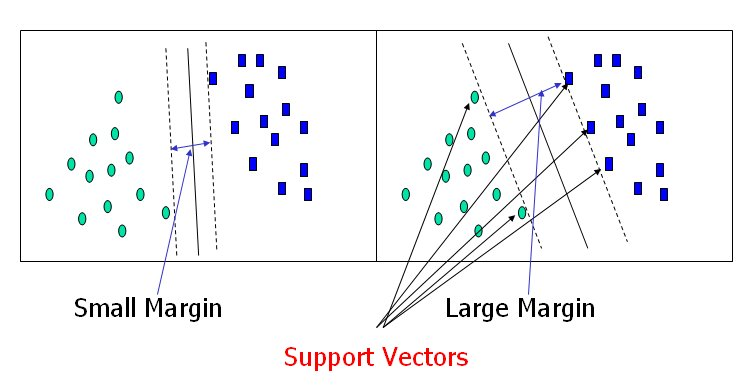
\includegraphics[width=\textwidth]{Figures/svm}
\decoRule
\caption[Support Vector Machines]{Support vector machines with their support vectors. \cite{svm}}
\label{fig:svm}
\end{figure}
\noindent In order to adapt Support Vector Machines to be able to fit non-lineair classifiers, some adjustments need to be done. This can be done with kernels. A kernel is a similarity function. The function compares two inputs and computes their similarity. Normally features are extracted from data and then fed into a machine learning algorithm. Kernels offer an alternative. The kernel should be a function to compare input data. The kernel, along with labeled data is then used to construct features. Using no kernel is called a lineair kernel. The basic type of kernel algorithms are called Gaussian kernels. The formula for Gaussian kernels is:
\begin{align}
K(x,y) = \exp{(\dfrac{-||x-y||^2}{2\sigma^2})}
\end{align}

\section{K-Nearest Neighbors}
The K-Nearest Neighbors or KNN algorithm is an algorithm which computes the classification by looking at the classes of the K-Nearest neighbors of the inputted data. The K-Nearest Neighbors is an Instance-based algorithm. \cite{mlcat} The chosen class is the class most common among its K-Nearest neighbors, this can be seen in Figure~\ref{fig:knn}. K is typically a small number. When K is equal to 1, the assigned class is the same as the class of the closest sample. \\\\
When training the algorithm, the input data and classes are stored. There are mutliple methods to compute the distance between data. Euclidean distance can be used for continous data. For discrete variables another metric can be used, such as the overlap metric or Hamming distance.\\\\
A major drawback of the KNN algorithm is the weakness to skewed data. Since the class is chosen based on the most popular nearest class, these popular classes may dominate the prediction. This can be overcome by taking the distance between the input data and the neighbors into account.
\begin{figure}[H]
\centering
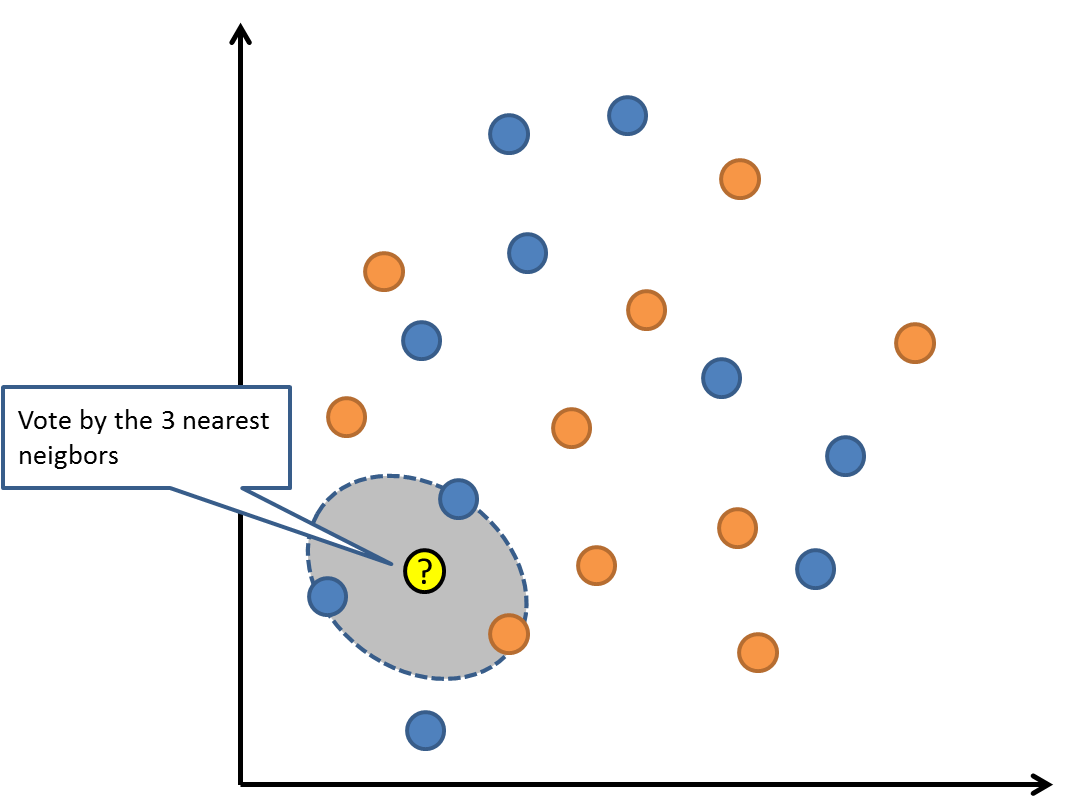
\includegraphics[width=0.8\textwidth]{Figures/knn}
\decoRule
\caption[K-Nearest Neighbors]{K-Nearest Neighbors. \cite{knn}}
\label{fig:knn}
\end{figure}

\section{Clustering}
Clustering is a machine learning concept using unsupervised learning. Unsupervised learning does not have labels with the training set. An unsupervised machine learning algorithm tries to find structure within the given training set. Clustering is the first type of unsupervised learning. It tries to cluster the training samples into different clusters.

\subsection{K-means Algorithm}
The K-means algorithm is a simple clustering algorithm. K is the number of clusters that is going to be used. The algorithm first randomly places the K clusters in the space (from the training set). This can be done by randomly chosing K training samples. Then it repeats the following steps until the cluster centers remain stationary. it iterates over all training samples, and assigns them to the closest cluster. Next the cluster centers are moved to the center of the total cluster. \\\\
The cluster centroids will be addressed using the symbol $\mu$ with $\mu_k$ the cluster centroid of cluster k. $c^{(i)}$ is the index of the cluster to which training sample  $x^{(i)}$ has been assigned. $\mu_{c^{(i)}}$ is the cluster centroid to which training sample $x^{(i)}$ has been assigned. The cost function can be described as:
\begin{align}
J(c, \mu) = \dfrac{1}{m} \sum\limits_{i=1}^m(|| x^{(i)} - \mu^{(i)}||)^2
\end{align}
The final clusters that are found by K-means are dependent on the random placement of the K clusters in the beginning. It could lead to suboptimal clustering. This can be fixed by running K-means a number of times and after each iteration check the value of the cost function to find the most efficient run of K-means. \\\\
There is a similar problem with determining the amount of clusters. The same method could be used to determine the correct number of clusters. However, manually determining the number of clusters could be more time efficient.
\section{Neural networks}
Neural networks are a useful alternative to logistic regression if the amount of features becomes too large. The origin of neural networks are algorithms which try to mimic the brain. There is a hypothesis, the "one learning algorithm" hypothesis, that shows that the brain can learn very different things, such as sound, touch, etc. by using a single algorithm. \\\\
A neural network is created of neurons, which are called a logistic unit. Each neuron receives input wires, and has an output wire, which computes a value using the sigmoid (logistic) hypothesis, the activation function. A neural network is a group of "neurons" that are connected together. This can be grouped into a layered approach as seen in Figure~\ref{fig:neuralnetwork}. The first layer is called the input layer, the final layer is called the output layer which outputs a $H_\theta(x)$ which is class. All layers inbetween these layers are called hidden layers.
\begin{figure}[H]
\centering
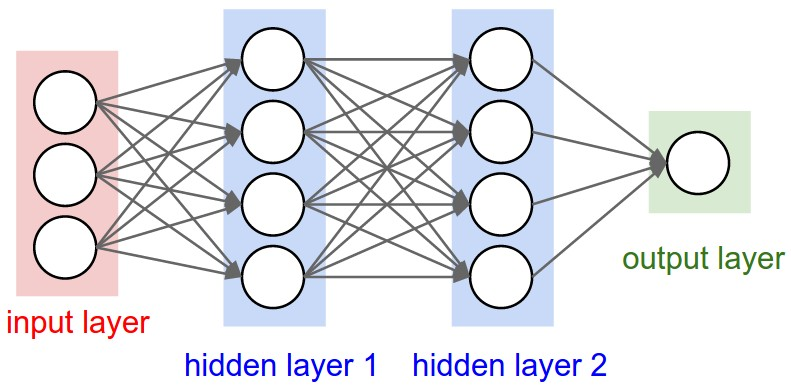
\includegraphics[width=1\textwidth]{Figures/neuralnet}
\decoRule
\caption[Neural network]{A neural network showing the different layers.\cite{neuralnetwork}}
\label{fig:neuralnetwork}
\end{figure}
\noindent Each logistic unit is denoted by $a_i^j$. $j$ is the layer and $i$ is the position in that layer. $\theta^j$ is a matrix of weights or parameters controlling function mapping from layer $j$ to layer $j+1$. $s_l$ is the number of units within a layer. The number of layers is denoted by $L$.\\\\The neural network works similar to logistic regression, except that it performs logistic regression from layer to layer. The parameters $\theta_j$ required are learned by itself. The architecture of a neural network refers to the way the units are connected to eachother. Neural networks can be used for multi-class classification. Hereby there are mutliple units in the output layer and each unit represents a different class. $K$ will denote the amount of output units.
\begin{figure}[H]
\centering
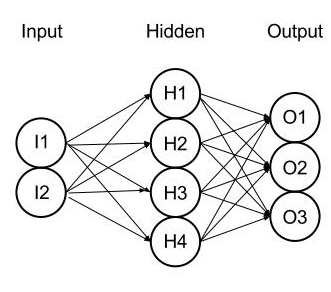
\includegraphics[width=0.7\textwidth]{Figures/neuralnetmulti}
\decoRule
\caption[Neural network with multi-class classification]{A neural network capable of multi-class classification. \cite{neuralnetworkmult}}
\label{fig:neuralnetworkmult}
\end{figure}
\noindent Data flows using the principle of forward propagation. The data passes through the first layers, move to the second layers and so on, until it arrives at the final layer. Mathematically this can be described as: 
\begin{align*}
a^{(1)} = x\\
z^{(2)} = \theta^{(1)}*a^{(1)}\\
a^{(1)} = g(z^{(2)})
\end{align*}
\subsection{Cost function and backpropagation}
The cost function for neural networks is a generalisation of the cost function for logistic regression. The cost function accounts for the different layers, units and the number of output units. To minimize the cost function, the same methods such as gradient descent can be used. However, the problem is how to compute the partial derivative of the cost function. Using backpropagation, it is possible to compute this. \\\\
The resulting class is known in the final layer. From here, the algorithm can find the error. $\delta_j^l$ will be the symbol used for the error of node $j$ in layer $l$. For an example with 4 layers:
\begin{align}
\delta_j^{(4)} = a_j^{(4)} - y_j\\
\delta^{(3)} = (\theta^{(3)})^T\delta^{(4)} * g'(z^{(3)})
\end{align}
The algorithm starts by setting a parameter $\Delta_{ij}^{(l)}$ to 0 for all $i$, $j$, $l$. Then, it iterates from $i=0$ to $m$, with $m$ the number of training samples. Each iteration, $a^{(1)}$ is set to $x^{(i)}$. Forward propagation is computed for $a^{(l)}$ for all $l = 2,3,..., L$. Using $y^{(i)}$, $\delta^{(L)}$ can be computed. Then the different $\delta^{(L-1)}$ to $\delta^{(2)}$ are computed. Finally, $\Delta_{ij}^{(l)}$ is incremented by $a_j^{(l)}\delta^{(l+2)}$ for each $l$. After the iteration is done, the final value for the partial derivative can be calculated: $\dfrac{\partial}{\partial \theta_ij^{(l)}} J(\theta)$. This can be done by dividing $\Delta_{ij}^{(l)}$ by the amount of training samples and adding $\lambda\theta_ij^{(i)}$. 
\subsection{Using a neural network}
A neural network should have as many input units as the dimension of features. The number of output units is equal to the number of classes. Default, there should be either 1 hidden layer or if there are more, all layers should have the same number of hidden units. The neural network should be trained by first assigning random weights to the values of $\theta$. Afterwards, forward propagation should be used to get $H_\theta(x^{(i)}$. Next the cost function should be computed. Backwards propagation is used to compute the partial derivatives. The result of backwards propagation can be checked by numerical methods to compute the gradient. Finally gradient descent or other advanced optimization methods with backpropagation should be used to try to minimize the cost function as a function to the parameters $\theta$.
\section{Dimensionality reduction}
Dimensionality reduction is the process of reducing the amount of features used in machine learning algorithms. This can be used to increase the accuracy and the performace of machine learning algorithms. One form is to do data compression. For example, transform 3D data into 2D data and eliminating a feature or dimension. It can also be used to reduce dimensions to be able to efficiently visualise data.

\subsection{Principle Component Analysis}
Principle Component Analysis is a way to do dimensionality reduction. The algorithm is formed as a minimalisation problem. When given N-dimensional data and N-1 dimensional data is prefered. The algorithm tries to find the correct N-1 dimensional value so that the projection is the closest to the original data. \\\\
Before this algorithm should be run, the features of the data should be scaled, so all features are on a similar scale. This can be done by using mean normalization. In order to reduce the dimension from $n$ to $k$ the covariance matrix should be computed:
\begin{align}
\Sigma = \dfrac{1}{m}\sum\limits_{i=1}^n((x^{(i)}) (x^{(i)})^T)
\end{align}
From this matrix, the eigenvectors need to be computed using singular value decomposition. From these values, only the first $k$ values are going to be used and be multiplied with the training data.\\\\
PCA can be used to speed up the time it takes for other learning algorithms to learn. By using PCA, the amount of features or the amount of training samples is reduced which reduces the running time of the training, but the compressed data still retains the same information as the uncompressed data.

\section{Anomaly detection}
Anomaly detection is also a form of unsupervised learning. The algorithm learns what normal behaviour looks like through the training set and then tries to predict if a given input data belongs to the normal behaviour or is abnormal for any reason.
\begin{figure}[H]
\centering
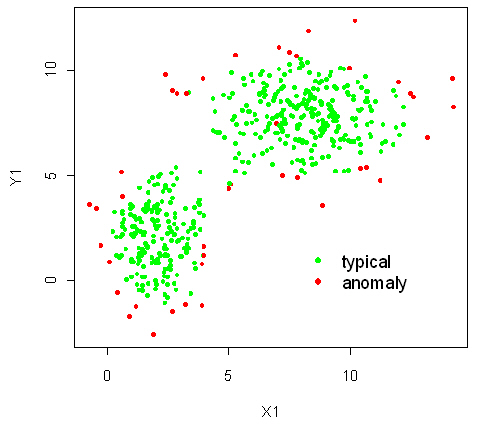
\includegraphics[width=0.8\textwidth]{Figures/anomaly}
\decoRule
\caption[Anomaly detection]{Anomaly detection. \cite{anomaly-fig}}
\label{fig:anomalydetection}
\end{figure}
\noindent Anomaly detection algorithms make heavy use of (Gaussian) Normal distribution:
\begin{align}
x \sim N(\mu, \sigma^2)
\end{align}
Hereby is $\mu$ the mean parameter and $\sigma$ is the standard deviation. Now the probability of $x$ being an anomaly can be calculated as:
\begin{align}
p(x) = \prod_{j=1}^n( \dfrac{1}{\sqrt{2\pi}\sigma_j} exp(- \dfrac{(x_j - \mu_j)^2}{2\sigma_j^2}) )
\end{align}

\section{Other algorithms}
There are also other, more specific and advanced categories of machine learning algorithms. There are decision tree algorithms, for example, Classification and Regression Tree (CART), Conditional Decision Trees, etc. There are Bayesian Algorithms which explicitly apply Bayes’ Theorem for problems such as classification and regression. These algorithms include Naive Bayes, Gaussian Naive Bayes, Multinomial Naive Bayes, etc. \cite{mlcat} \\\\
Association Rule Learning Algorithms are methods that extract rules that best explain observed relationships between variables in data. Apriori algorithm and Eclat algorithm are examples of such algorithms. Deep Learning Algorithms are a modern modification to Artificial Neural Networks that exploit abundant cheap computation. Deep learning networks are very deep and complex neural networks. Deep Boltzmann Machine (DBM), Deep Belief Networks (DBN) and Convolutional Neural Network (CNN) are examples of deap learning algorithms.  \cite{mlcat}\\\\
Ensemble Algorithms such as Bootstrapped Aggregation (Bagging) are models that combine multiple weaker models and try to combine the predictions made by these models. Yet there are still many more algorithms.  \cite{mlcat}\\\\
A lot of algorithms are specifically constructed for a specific sub-field of machine learning, for example computer vision, natural language processing, etc. Even within the categories of algorithms that were discussed, regression, regularization, instance-based, clustering, neural networks and dimensionality reduction, there are a lot of different variants. However, these are considered to be to advanced and outside the scope of this thesis. 

\chapter{Machine Learning Techniques}

\section{Dimensionality reduction}
Dimensionality reduction is the process of reducing the amount of features used in machine learning algorithms. This can be used to increase the accuracy and the performace of machine learning algorithms. One form is to do data compression. For example, transform 3D data into 2D data and eliminate a feature or dimension. It can also be used to reduce dimensions to be able to efficiently visualise data.\\\\
Dimensionality reduction can be used to speed up the time it takes for other learning algorithms to learn. By using dimensionality reduction, the amount of features or the amount of training samples is reduced which reduces the running time of the training, but the compressed data still retains the same information as the uncompressed data.

\subsection{Principle Component Analysis}
Principle Component Analysis is a way to do dimensionality reduction. The algorithm is formulated as a minimalisation problem. When given N-dimensional data and N-1 dimensional data is prefered, the algorithm tries to find the correct N-1 dimensional value so that the projection is the closest to the original data. \\\\
Before this algorithm is run, the features of the data should be scaled, so that all features are on a similar scale. This can be done by using mean normalization. In order to reduce the dimension from $n$ to $k$ the covariance matrix should be computed. \\\\
From this matrix, the eigenvectors need to be computed using singular value decomposition. From these values, only the first $k$ values are going to be used and be multiplied with the training data.

\section{Anomaly detection}
Anomaly detection is also a form of unsupervised learning. The algorithm learns what normal behaviour looks like through the training set and then tries to predict if a given input data belongs to the normal behaviour or is abnormal for any reason. \\\\
In Figure~\ref{fig:anomalydetection}, the algorithm has been trained using the green data points. These make up the normal behaviour. The algorithm can then predict whether a data point is normal, or an anomaly. It seems very close to One-class SVM's as seen in Section~\ref{oneclassSVM}. However, One-class SVM's are used for simple binary classification. Normal behaviour of a systems typically does not fall within a single class. Usually many different classes make up normal behaviour. 
\begin{figure}[H]
\centering
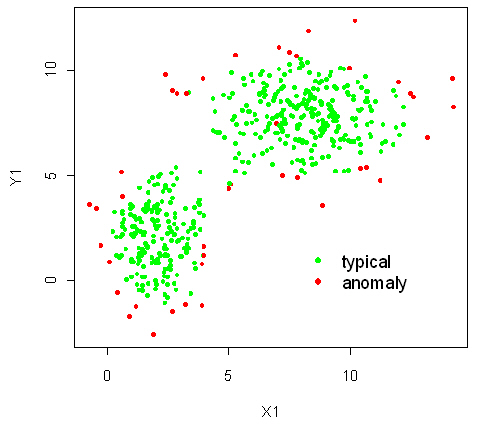
\includegraphics[width=0.8\textwidth]{Figures/anomaly}
\decoRule
\caption[Anomaly detection]{Anomaly detection. \cite{anomaly-fig}}
\label{fig:anomalydetection}
\end{figure}

\noindent Anomaly detection is useful when there are a lot of data points belonging to normal behaviour and there are almost no abnormal behaviour data points. General supervised learning algorithms are usefull when there are a lot of data points of both normal and abnormal behaviour. \cite{anomalyCoursera}

\subsection{Normal Distribution}
\noindent Anomaly detection algorithms make heavy use of (Gaussian) Normal distribution:
\begin{align}
x \sim N(\mu, \sigma^2)
\end{align}
Hereby $\mu$ is the mean parameter and $\sigma$ is the standard deviation. Now the probability of $x$ being an anomaly can be calculated as:
\begin{align}
p(x) = \prod_{j=1}^n( p(x_j ; \mu_j, \sigma_j)  ) \\
p(x_j ; \mu_j, \sigma_j) = \dfrac{1}{\sqrt{2\pi}\sigma_j} exp(- \dfrac{(x_j - \mu_j)^2}{2\sigma_j^2}) 
\end{align}
\noindent $p(x_j ; \mu_j, \sigma_j)$ is the probability of $x_j$ with a Normal Distribution with parameters $(\mu_j, \sigma_j)$. $p(x)$ is the product of all these probabilities. The formula for the probability is the probability density of the Normal distribution. This function is plotted in Figure~\ref{fig:normalExample}. The $y$-axis is the density function, the $x$-axis is the $x$ value in the formula. 

\begin{figure}[H]
\centering
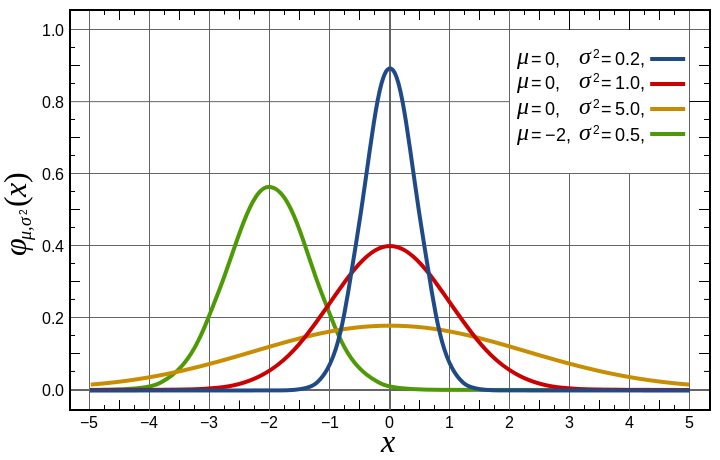
\includegraphics[width=0.8\textwidth]{Figures/normaldist}
\decoRule
\caption[Normal Distribution]{Normal Distribution. \cite{normalExample}}
\label{fig:normalExample}
\end{figure}

\section{Online learning}
Online learning is a technique to update an algorithm. Instead of feeding all data to the learning algorithm, the data is fed incrementally. The algorithm can keep learning from data even after it has initially learned a model. \\\\
Some algorithms such a KNN are immediatly able to do online learning. Other algorithms, such as SVM need to be slightly altered in order to be able to do online learning. \\\\
Online learning is very useful when the data is dependent on the time. For example, stock prices prediction. The data that is used to train an algorithm today might be able to predict stocks for tomorrow, but it is not very effective at prediction the stock market at long term. That is why it is useull to be able to keep training the algorithm. \cite{onlineLearning}

\section{Bagging}
Bagging is a technique which tries to create new datasets from a given data set. It takes a data set as input and generates multiple slight variations of the data in the given data set. These slight variations are used to construct new data sets. This method is also called Bootstrapped Aggregation, or bagging for short. \\
\\
Once multiple data sets have been generated, it is possible to combine multiple weaker models and training algorithms and try to combine the predictions made by these algorithms. This is useful to deal with unstable data. Unstable data is data that can give different results depending on the algorithm that is used to process the data. An example of bagging and Neural Networks can be seen in Figure~\ref{fig:baggingExample}. \cite{mlcat}

\begin{figure}[H]
\centering
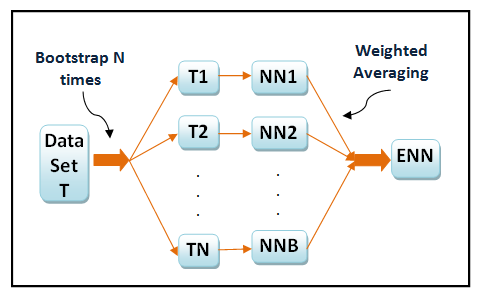
\includegraphics[width=0.8\textwidth]{Figures/bagging}
\decoRule
\caption[Bagging example with Neural Networks]{Bagging example with Neural Networks. \cite{baggingExample}}
\label{fig:baggingExample}
\end{figure}
\chapter{Validating an algorithm}

\section{Machine learning evaluation}
Machine learning diagnostics are tests that can be run to get to know what is and isn't working with a machine learning algorithm. They also provide guidance as to how performance could be improved. 

\section{Error analysis}
\label{errorAnalysis}
When trying to use machine learning for any purpose, such as intrusion detection systems, there are several considerations to be made. Another important step is the approach used to find the correct algorithm. 
The recommended approach is to start with a simple algorithm and test it with cross validation data. Afterwards, learning curves could be plotted to decide if more or less data, more or less features, ... are likely to help. Finally, error analysis can be done by maually examining the samples on which the algorithm made mistakes. This could help to spot any systematic trends in the type of samples on which the algorithm is making mistakes.\\\\
The error analysis mostly consists of manual or brute force work. The samples on which the algorithm is wrong need to be categorized based on which features could help it categorize correctly and on which class it belongs to. Calculating statistics, such as the accuracy of the algorithm can also help with error analysis. It is possible to brute force this approach by automatically trying a lot of different combinations of features. This is less efficient than manually tweaking the algorithm.\\\\
Another issue to account for are skewed classes. Skewed classes are classes that are underrepresented in training data. For example, in binary classification, when trying to classify a flow as malicious or not, the training set might only provide $0.5$\% malicious data. Knowing this, having an accuracy of $99$\% does not seem that great.

\begin{figure}[H]
\centering
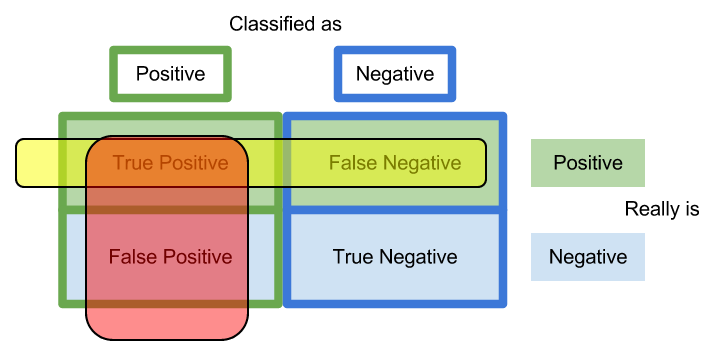
\includegraphics[width=0.9\textwidth]{Figures/precisionrecall}
\decoRule
\caption[Precision and recall]{Precision and recall. \cite{recall-fig}}
\label{fig:precisionrecall}
\end{figure}
\noindent A different metric is required to evaluate machine learning algorithms that are trained using skewed data. This metric is the precision and recall method. We classify a result as true positive, true negative, false positive and false negative. False positive and false negative respectively mean that the predicted value is falsely classified as positive and negative. These are the errors. True positive and true negative are correctly predicted values. \textbf{Precision} is defined as the fraction of predicted malicious flows that were actually malicious: 
$$\dfrac{true positive}{true positive + false positive}$$
\textbf{Recall} is defined as the fraction of predicted positives and the actual amount of positives: 
$$\dfrac{true positive}{true positive + false negative}$$
There is always a tradeoff to be made between precision and recall. As an effect of a higher precision, there will be a lower recall. Similarly, a higher recall means a lower precision.\\\\
Algorithms with a different precision and recall can be compared to eachother. This can be done using an F-score: 
$$2 \dfrac{PR}{P+R}$$
\noindent The F-score is the harmonic mean of precision and recall. For Table~\ref{tab:precrecal}, this means that Algorithm 1 is the most effective. In contrast, using for example the average of both precision and recall would make Algorithm 3 the most effective.\\\\
The main reason to use the harmonic mean is because the average is taken of
ratios (percentages), and in that case the harmonic mean is more appropriate than the (arithmetic) mean. \cite{harmonic}
\begin{table}[H]
\caption{Example of precision and recall of certain algorithms.}
\label{tab:precrecal}
\centering
\begin{tabular}{| l | c  r|}
\toprule
\tabhead{} & \tabhead{Precision (P)} & \tabhead{Recall (R)}\\
\midrule
Algorithm 1 & 0.5 & 0.4\\
Algorithm 2 & 0.7 & 0.1\\
Algorithm 3 & 0.02 & 1.0\\
\bottomrule
\end{tabular}
\end{table}
\noindent Looking at the values of the precision and the recall in Table~\ref{tab:precrecal}, it can already intuitively be seen that Algorithm 1 is the best algorithm. For algorithm 3, the precision is 0.02, which means that there were a lot more false positives than true positives. With a recall of 1.0, there are almost no false negatives. This means that almost every prediction was a positive. That is not good at all. \\\\
Algorithm 2 has similar problem but the other way around. Only Algorithm 1 seems to have some kind of balance between precision and recall which makes it seem as the best algorithm. This confirms that the F-score is a better metric than the average.
\begin{table}[H]
\caption{Example of average and F-score of certain algorithms.}
\label{tab:avgscore}
\centering
\begin{tabular}{| l | c  r|}
\toprule
\tabhead{} & \tabhead{Average} & \tabhead{F-score}\\
\midrule
Algorithm 1 & 0.45 & 0.444\\
Algorithm 2 & 0.4 & 0.175\\
Algorithm 3 & 0.51 & 0.039\\
\bottomrule
\end{tabular}
\end{table}
\noindent The data that is being fed into a machine learning algorithm is also important to consider. Sometimes a lot of data can be useful. First, the assumption is made that the features are chosen correctly and sufficiently. Lots of data is useful when a machine learning algorithm is used with a lot of parameters such as a neural network with a lot of hidden units. This means that the algorithm has low bias. 

\subsection{Different Algorithms}
If the number of features is large relative to the number of training samples, then using a lineair kernel Support Vector Machine or logistic regression is preferred. A Gaussian kernel is preferred when there are more training samples than features, but the difference is rather small. Otherwise, new features should be added. Neural networks are almost always effective but they may be slower to train.

\subsection{Evaluating the hypothesis}
\label{evaluationHypothesis}
The most obvious way to test whether the hypothesis is correct is by dividing the training set into two sets. The first set which should have approximatly 70\% of the samples of the original training set will be used to train the learning algorithm. The other set is used to check whether the output of the learning algorithm is correct. After the algorithm has done its learning with the training set, this check set is thrown into the algorithm. Aftwards the output of the algorithm is compared to the labels of the check set. If the output isn't correct, a test error can be computed. These test errors can be used to compute global error value, which could be calculated by, for example, a mean squared error. This value can be used ito evaluate the hypothesis. \cite{evalml}

\subsection{Model selection algorithm}
\label{modelselection}
To get back to the problem of overfitting, there is another method next to regularisation called model selection. Model selection uses the same principle as mentioned above except it divides the training set into three new sets. A new training set, a cross validation set and a test set. \\\\
The training set is used to actually train the algorithm. The cross validation set is used to compare different algorithms or different models. Different models can be tested and compared to eachother by comparing the cross validation error, the error between the prediction and the actual output from the cross validation set. The testing set is used purely to test the algorithm once the cross validation has been done. It is considered good practice to use seperate sets for cross validation and testing. \cite{wiki}

\subsection{Diagnosing bias vs variance}
High variance means that there is an overfitting problem. High bias on the other hand, is the opposite problem. It means that the hypothesis does not fit the training set at all. There is a relation between the amount of training samples and the training error. With more training data, the training error goes down. \\\\
With a low model complexity, there is a high error for the training set and a high error on the test set. This is a signal there is a underfitting problem or a high bias problem. It does not help to increase the amount of training samples since the model just is not complex enough. \\\\
With a high complexity model, the training set error is very low, but the test set error is very high. This is a signal there is an overfitting problem or a variance problem. This can be seen in Figure~\ref{fig:trainingsamples}. The complexity of the model can be adjusted by changing the amount of features that are being used. \cite{stanford}

\begin{figure}[H]
\centering
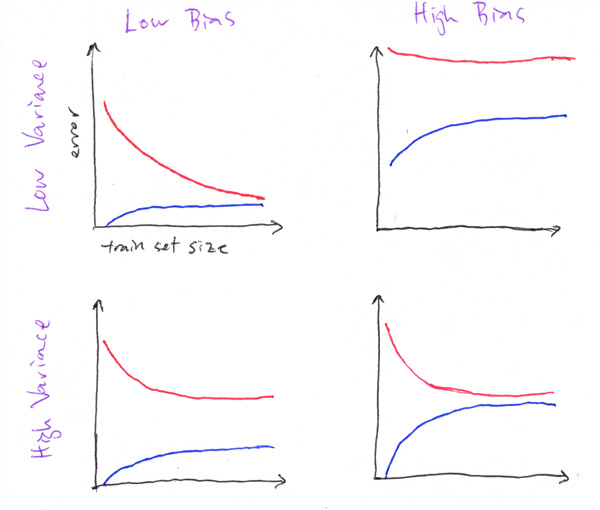
\includegraphics[width=0.8\textwidth]{Figures/bias_variance_chart}
\decoRule
\caption[Training samples comparison]{The effect of the amount of training samples on the accuracy.}
\label{fig:trainingsamples}
\end{figure}
\noindent In Figure~\ref{fig:trainingsamples} the general trend of training error and test (or true) error is shown. This figure shows the example for high bias and no matter how many training samples there are, the functions are already converged to the same error amount.\\\\
In contrary to high bias, high variance can be solved by using extra training samples. In that case there is a gap inbetween the true error line and the training error line and it is likely that they still converge to the same point. With a bigger training set, they converge more and more. These curves are called learning curves.


% Chapter 1

\chapter{Machine learning for an IDS} % Main chapter title

\label{Chapter3} % Change X to a consecutive number; for referencing this chapter elsewhere, use \ref{ChapterX}

\section{Using ML for an IDS}
An intrusion detection system has to detect whether some data it receives is either malicious or regular web traffic. This can be seen as a classification problem which means an machine learning algorithm for classification could be used. It needs to be determined whether data is either normal network traffic or malicious behaviour. \\
\\
Some parameters have to be chosen that will be feed into the machine learning algorithm.

\section{Disadvantages of using ML for an IDS}
\subsection{Problems}
As said before, machine learning for an intrusion detection system is a classification problem. More precisely, it can be said that intrusion detection systems have to detect abnormal behaviour in a network with mostly normal behaviour. There are several problems that can be encountered when using machine learning techniques.\\
\\
The first problem is the ability to detect new attacks. A machine learning algorithm compares incoming data with a model that it has created internally. An new type of malicious behaviour might appear to be closer to normal network traffic as compared to the model of known attacks. \\
\\
Another problem is the diversity of network traffic. The notion of "normal network traffic" is difficult to actually define. The bandwidth, duration of connections, origin of IP addresses, applications used can vary enormously through time. This makes it quite difficult for machine learning algorithms to distinguish between "normal network traffic" and malicious behaviour.\cite{ClosedWorld} 

\subsection{Solutions}
There are several solutions that can be used in order to make machine learning algorithms more effective for intrusion detection systems. One option is to chance the way the classification problem is defined. Instead of defining the classes, "normal" and "malicious", there might be different classes for different types of malicious behaviour. In the same way, different classes can be defined for different types normal traffic. 

% Chapter Template

\chapter{IP Flows} % Main chapter title

\label{flow} % Change X to a consecutive number; for referencing this chapter elsewhere, use \ref{ChapterX}

\label{export}
Flows are aggregated from all packet data that travels through the network. Flow exporters are programs which collect network packets and aggregate them into flow records. A flow is not the same as a TCP connection. A flow can be any communication between two devices with any protocol. Flows are defined using a (source\_IP, destination\_IP, protocol) tuple. This is why flows are also called IP Flows.\\
\\
Since flow data does not contain any payload information, intrusion detection systems that use flow data cannot detect malicious behaviour embedded within payload data. \cite{IPFlow}

\section{How to use flow-data}
The following attributes are available with flow-data:
\begin{itemize}
\item Source IP
\item Destination IP
\item Protocol name
\item Source port
\item Destination port
\item Starting time of the flow
\item Duration of the flow
\item Amount of packets in the flow
\item Amount of bytes in the flow
\end{itemize}
However, should a flow exporter be implemented, some additional features can be generated from packet data. \ref{export}
\begin{itemize}
\item Amount of TCP SYN within the flow
\item Source and Destination Type of Service
\item Payload size
\end{itemize}
These data can be used within the machine learning algorithms. However some variables have undesirable effects on the accuracy of the algorithm. Some care should be taken when training the machine learning algorithms with the additional data. Not all data, both training data as predictive data, will have the additional features.\\
\\
Most machine learning libraries use numeral data instead of string data. All string data has been hashed in order to be able to use it in machine learning algorithms. The probability on a collision is low enough to be able to ignored.

\subsection{IP addresses}
Flow data can contain multiple forms of IP addresses. Both IPv4 and IPv6 data can be found. For some protocols the flow data can also contain the MAC-addresses instead of the IP-address. These addresses are hashed, so they become numeral, discrete data and are then fed into the machine learning algorithm.\\
\\
Using the IP, it is possible to find the country or region of origin. Tests where the country of origin was fed into the machine learning algorithms, have been done. Results however showed, that the accuracy of the IDS became lower.

\begin{table}[H]
\caption{The effects of using IP country-of-origin on accuracy of IDS.}
\label{tab:country}
\centering
\begin{tabular}{l l l}
\toprule
\tabhead{With Country-of-origin} & \tabhead{Accuracy}\\
\midrule
Yes & 96.16\%\\
No & 98.57\%\\
\bottomrule\\
\end{tabular}
\end{table}

\subsection{Ports and protocol name}
Both the source and destination port are discrete data. They are usually received in decimal form, however some data-sets might use them in hexadecimal data or refer to ports as "ssh port" instead of "22". Port data, in decimal form, can be directly fed into the machine learning algorithm.\\
\\
The protocol name can simply be converted to a standard string in lower case, in order to avoid errors by lower and uppercase forms of the same name (for example "tcp" and "TCP"). This string can than be hashed into a discrete value.

\subsection{Timing}

\subsection{Size} 
The amount of packets used in the flow and the amount of bytes are both discrete data. They are always received in decimal form. They can immediately be fed into the machine learning algorithm.

% Chapter Template

\chapter{Implementation} % Main chapter title

\label{implementation} % Change X to a consecutive number; for referencing this chapter elsewhere, use \ref{ChapterX}

\begin{itemize}
\item Discuss important decisions
\item Talk about the data sets
\end{itemize}

\begin{itemize}
\item Cegeka
\item CTU datasets
\item Own generation + inline placement
\end{itemize}

\section{Structure}

\section{Class diagram}
% Chapter Template

\chapter{Evaluation} % Main chapter title

\label{evaluation} % Change X to a consecutive number; for referencing this chapter elsewhere, use \ref{ChapterX}

In this chapter, the different machine learning algorithms are evaluated. In Section~\ref{datasets}, the different evaluation steps are explained. There are four steps. Step one is the training of the machine learning algorithm, this is evaluated using learning curves. Step two is evaluation within the same dataset, this is done using the CTU dataset. In the third step, cross-dataset validation is done. The algorithms are evaluated by using multiple datasets containing real-world data. In the final step, unlabeled real-world data is used. \\
\\
For the first and second step, the algorithms are always trained using a subset from the datasets and tested using another subset. Since the datasets contain a lot of different labels (and thus classes), it has been chosen not to always follow the "30/70" rule as explained in Section~\ref{evaluationHypothesis}. Instead the algorithm is trained using the number of training samples that indicates a good accuracy in the learning curves, and tested using a set of $~230000$ samples. This number was found by looking at all the learning curves from the different algorithms and choose the appropriate training size. From these training sizes, the largest value was chosen and on this value the "30/70" rule was used. This was done to make sure that every experiment was tested using the same amount of samples and that for each experiment the balance between training and testing samples was at least "30/70". This is done to allow statistically correct comparisons to be made across different machine learning algorithms. Each training set also contains an about even split between malicious and non-malicious samples. The samples themselves are chosen at random from the datasets.\\
\\
In the third step, the algorithm is trained using samples from both the CTU dataset and the SQL dataset. The amount of training and testing samples are calculated on the same way as they were calculated for the first and second step. The SQL dataset has not been used in the second step. This dataset only contains malicious samples, most of these samples are also ssh scans. This means that when the machine learning algorithm is only trained using data from this dataset, it only knows what an ssh scan looks like, and predicts that everything is a ssh scan since it does not know any other classes. \\
\\
In the fourth step, the algorithm is evaluated using real-world data. This is done using the Cegeka and EDM dataset. The Cegeka dataset also contains firewall logs, which have been used to check the performance of the algorithm. The EDM dataset has also been used and the samples have manually been checked. This was a tedious and slow task and the reason that not many samples have been used from this dataset. In total $10000$ samples were used from the EDM dataset. \\
\\
The verification that was done only verified whether the flow was malicious or non-malicious. The exact class that was predicted has not been verified. This means that a flow could be labeled as a google-analytics flow but in reality could be some other non-malicious flow. This manual check was done by using the labeled data sets and comparing the flows manually. The SSH scans within the SQL dataset all look very similar. It can be seen whether the flow looks similar or not. For example, an indicator that was used was the amount of packets and the amount of bytes in a flow. Other indicators were the protocol that was used and the TCP flags that were set. For the botnet traffic, an easy indicator was the whether the flow was outgoing or incoming. The botnet traffic in the dataset was often outgoing. If it wasn't it was always characterised by having a low amount of packets ($ <= 2$) and a low amount of bytes ($ < 500 $).\\
\\
As explained in Section~\ref{featureSelection}, there are several ways to choose features. All these different ways have been used in the experiments. In order to remove the factor that chance might play a role in the experiments, each experiment has been \textbf{run 10 times}. In total, more than a thousand experiments were done. The results have been averaged, and the variance is calculated to assess statistical relevance.\\
\\
In order to evaluate the machine learning algorithms, some metrics need to be used. The F-score as explained in Section~\ref{errorAnalysis} is used. The F-score is always a number between $0$ and $1$, indicating a percentage. The F-score can be used in several ways. Either it can be used to evaluate how well a machine learning algorithm can distinguish between malicious and non-malicious flows, or it can be used to evaluate how well the algorithm can classify flows.\\
\\
In order to use the F-score to evaluate how well a machine learning algorithm can distinguish between malicious and non-malicious flows, the intrusion detection needs to happen binary. All that needs to be known is whether a flow is malicious or it is not. In order to calculate the F-score, it needs to be known what a true positive and true negative is. A true positive is defined as a malicious flow, a true negative is defined as a non-malicious flow. This type of F-score will be called the \textbf{binary F-score} in this thesis.\\
\\
The F-score can also be used to check how accurate the machine learning algorithm can predict the correct class. The interest here is in multi-class classification. This F-score will be called the \textbf{multi-class F-score}. A flow is positive when it belongs to the correct class, and negative when it does not belong to the correct class.\\
\\
In the implementation, multi-class classification is used. The machine learning algorithm predicts the actual class of a flow. The implementation also has a list which contains all classes that are considered non-malicious. Using this list, it can be calculated whether the class that was predicted means that the flow is malicious or non-malicious. \\
\\ 
A high binary F-score does not mean that the multi-class F-score is also high. The machine learning algorithm might be able to distinguish between malicious flows and non-malicious flows, but might not see the difference between different anomalies.\\
\\
\textbf{A baseline} needs to be established. Comparing each machine learning algorithm, a best algorithm might be found. However, if the algorithm does not perform better than the baseline, the algorithm does not perform well. Two baselines have been used in this thesis. The first baseline predicts the classification randomly. This is used to know whether a machine learning algorithm can predict the actual class better than randomly. The other baseline always predicts a non-malicious class. This baseline is used since the non-malicious samples outnumber the malicious samples. This means that having a couple false negatives is worse than a couple false positives. \\
\\
Another metric that has been used are \textbf{learning curves} as seen in Figure~\ref{learningcurve}. These cannot be used to measure the performance as they only show the accuracy of the algorithm. The \textbf{accuracy} is the percentage of correctly classified flows. The reason that it cannot be used to measure the performance is because the accuracy is not an accurate representation of the performance. For example, the accuracy might be $99$\%. However it might be possible that every sample was classified as one of the non-malicious classes. This means that even though the accuracy is $99$\%, the algorithm cannot detect any malicious behaviour.\\
\\
In order to construct the learning curve, a subset is chosen from the datasets. The subset is chosen such that the distribution of the labels is kept. The size of the subset depends on which algorithm is being evaluated and how long it takes for that algorithm to train. In each iteration in the construction of the learning curve, random samples are chosen to create the training set during that iteration. This has as effect that not necessarily every label appears in the training set. For this reason, it was chosen to use the accuracy in the learning curve and not the F-score. Since these F-scores are not necessarily a good representation of the F-scores that are found in the other experiments. Even though the training set might not contain every label, the constructed learning curve can still show signs of overfitting or underfitting. \\
\\
Figure~\ref{fig:randombaseline} shows an example of a learning curve. The lines show how the accuracy behaves when the amount of training samples are increased. The $y$-axis shows the accuracy as a number between $0$ and $1$ which indicate a percentage. The lightly colored areas are calculated using a standard deviation. The red line represents the training score. This is how accuratly the algorithm can make predictions on the data that was used to train the algorithm. The green line, is data that is used for cross-validation. This is data that was not used for training. The learning curves of the baselines have been included in all learning curve graphs.\\
\\
It can be seen that in the beginning the random baseline has a higher accuracy than when more training samples are used. It would be expected that the random baseline  has the same accuracy across different sizes of training samples. However, the random baseline can only predict labels that appear in the training set. Since some labels are skewed, they may not appear in the training set. Because of this, the random baseline will predict only the non-skewed labels and have a slightly higher accuracy. When the training set is larger, the chance that not every label appears in the training set is very small. The effect of this is also very small, with just a difference of $0.8$\%. The training sets used for the normal experiments are casefully chosen so that every label appears in high quantities in order to properly train the algorithms. \\
\\
For the learning curves, this does not matter, since the learning curve will look the same and still show the signs of overfitting and underfitting. This has been verified by manually constructing a learning curve. The library used for the implementation uses the random approach when constructing learning curves and also immediatly shows the standard deviation. The library can also construct these learning curves faster and uses a lot of iterations. 

\begin{figure}[H]
\centering
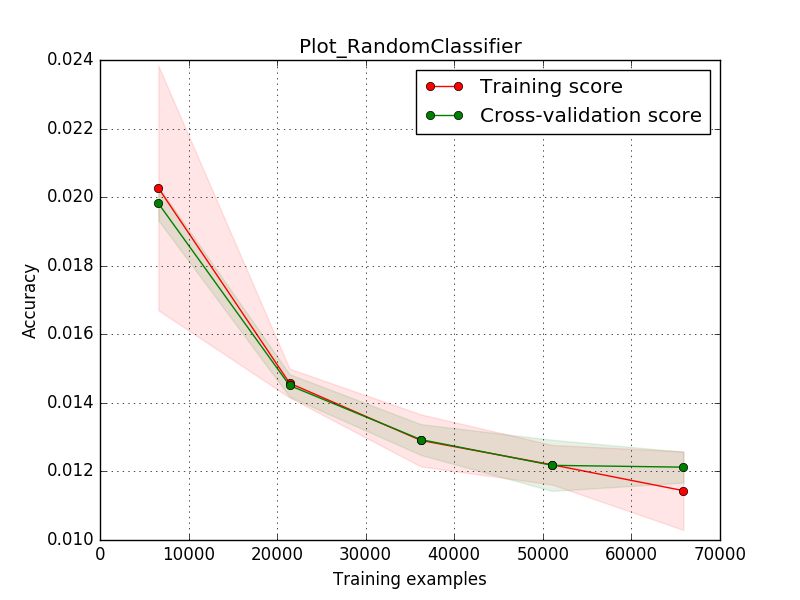
\includegraphics[width=0.6\textwidth]{Figures/Plot_RandomClassifier}
\decoRule
\caption[Random Baseline learning curve]{Random Baseline learning curve}
\label{fig:randombaseline}
\end{figure}

\noindent In Table~\ref{tab:baselinerandom} and Table~\ref{tab:baselinepositive} the scores are listed. The binary precision of Table~\ref{tab:baselinepositive} would give a divison by zero. If that is the case, the score is set to $0.0$. Both F-scores in both baselines are low. The random algorithm is terrible at classification. The closer to $0$ the F-score is, the less well the algorithm performs. The tables also list the amount of samples used, aswell as the binary classification. This is done to show how many samples were used in the test. The amount of positive and negative training samples is also shown. Finally, the variance is shown. This shows how much the F-scores fluctuate in the different experiments that were done.

\begin{table}[H]
\begin{minipage}{0.5\textwidth}
\caption{Baseline Random classifier (uniform): Average.}
\label{tab:baselinerandom}
\centering
\begin{tabular}{l r}
\toprule
Multi-class F-score & 0.0162 \\
Multi-class Precision & 0.1205 \\
Multi-class Recall & 0.0096 \\
\midrule
Binary F-score & 0.4653 \\
Binary Precision & 0.3592 \\
Binary Recall & 0.6603 \\
\midrule
Total amount of samples & 231797.0 \\
False negative & 28278.0 \\
False positive & 98054.15 \\
True negative & 50492.85 \\
True positive & 54972.0 \\
\midrule
Positive training samples & 82159.0 \\
Negative training samples & 49638.0 \\
\midrule
Variance Multi-class F-score & 1.18e-07 \\
Variance Multi-class Precision & 8.33e-06 \\
Variance Multi-class Recall & 4.46e-08 \\
\midrule
Variance Binary F-score & 8.21e-07 \\
Variance Binary Precision & 5.00e-07 \\
Variance Binary Recall & 2.48e-06 \\
\bottomrule
\end{tabular}
\end{minipage}
\begin{minipage}{0.5\textwidth}
\caption{Baseline Random classifier (All negative): Average.}
\label{tab:baselinepositive}
\centering
\begin{tabular}{l r}
\toprule
Multi-class F-score & 0.0287 \\
Multi-class Precision & 0.1104 \\
Multi-class Recall & 0.0183 \\
\midrule
Binary F-score & 0.0 \\
Binary Precision & 0.0 \\
Binary Recall & 0.0 \\
\midrule
Total amount of samples & 231797.0 \\
False negative & 83250.0 \\
False positive & 0.0 \\
True negative & 148547.0 \\
True positive & 0.0 \\
\midrule
Positive training samples & 0.0 \\
Negative training samples & 49638.0 \\
\midrule
Variance Multi-class F-score & 3.41e-07 \\
Variance Multi-class Precision & 4.51e-06 \\
Variance Multi-class Recall & 1.14e-07 \\
\midrule
Variance Binary F-score & 0.0 \\
Variance Binary Precision & 0.0 \\
Variance Binary Recall & 0.0 \\
\bottomrule
\end{tabular}
\end{minipage}
\end{table}

\section{K-nearest Neighbors}
\label{eval:knn}
K-nearest Neighbors as seen in Section~\ref{algorithm:knn} is a very promising algorithm for intrusion detection. $k$ was chosen at the default value of $5$.  However, different experiments have been done to compare the effect of $k$ on the perofrmance of the machine learning algorithm. The default distance metric that was used, is the Manhattan distance. In a realistic data-set, the malicious data is skewed. For this reason, the solution proposed in Section~\ref{knn:sol} was used. The first experiment that was done, was to construct the learning curve as seen in Figure~\ref{fig:knnlearn1}. \\
\\
Since KNN uses the $k$-closest neighbors and their distance to the to-be-predicted data point, it is normal that the training score is $1.0$. This is because the training score is calculated by feeding the training data to the machine learning algorithm to test it. The closest point to any training data point is that data point itself. This means that the algorithm will predict the same class. Overfitting is unlikely. In that case, the training score is expected to be high, but the cross-validation score should go down. It can be seen that the algorithm converges to an accuracy of about 86\%, but the algorithm shows a general trend to improve the accuracy when more training data is used. Underfitting is also unlikely because of this trend. 

 \begin{figure}[H]
\centering
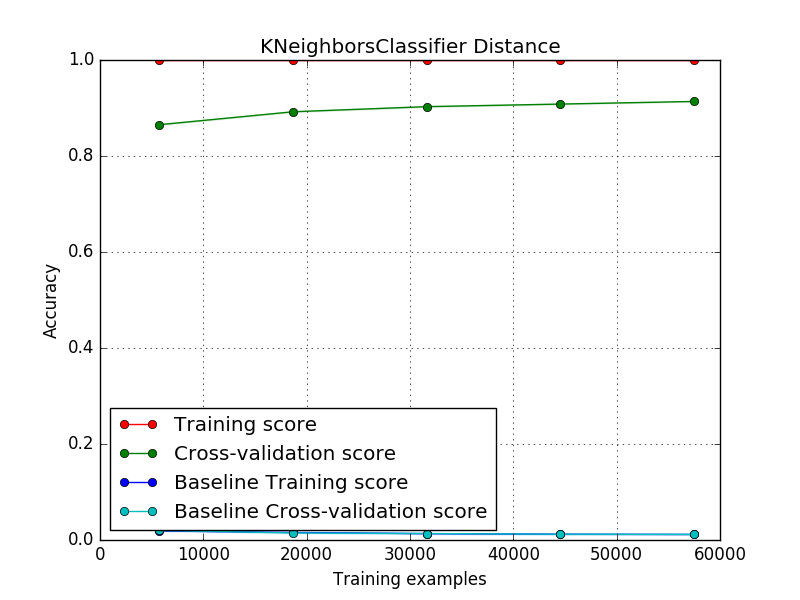
\includegraphics[width=0.6\textwidth]{Figures/KNeighborsClassifier_Distance}
\decoRule
\caption[Learning Curve for K-Nearest Neighbors]{Learning Curve for K-Nearest Neighbors}
\label{fig:knnlearn1}
\end{figure}

\noindent The first experiment using the F-score that has been done was a validation within the CTU dataset. This is shown in Table~\ref{tab:knn:ctu}. The experiment was done with all three feature sets. The algorithm was trained using $\sim80000$ samples with about as much malicious and non-malicious data. First the general results are discussed. Afterwards the different feature sets are discussed.\\
\\
The variance on both F-scores are very low, which means that the average result is statistically relevant. The binary F-score is $\sim0.9500$ is quite high. This means that the algorithm is able to distinguish between malicious and non-malicious data. The multi-class F-score is lower, which means the algorithm does make more mistakes concerning the exact classification. Together this means that the malicious data is grouped together, but the actual classes within the malicious data are less distinguishable. \\
\\
The effect of using the country of origin does not seem to have a lot of impact on the results. This could be due to the fact that the data belongs to a data set which contains data from mosty the same country. Using TCP flags does increase the performance immensely.  This means that the different classes do become more distinguisable when more data, and more specifically the TCP flags, are used. KNN uses the $k$-closest neighbors and their distance to the to-be-predicted data point. Because of the high binary and multi-class F-score, it can be said that most classes and more specifically, the malicious and non-malicious samples are grouped together. If different samples weren't grouped together, then the $k$-closest neighbors would be of different classes, and the F-score would be much lower.

\begin{table}[H]
\caption{K-Nearest Neighbors: comparing different feature sets: CTU-dataset}
\label{tab:knn:ctu}
\centering
\begin{tabular}{l c c r}
\toprule
Feature set & Standard & TCP & Country \\
\midrule
Multi-class F-score & 0.6153 & 0.8476 & 0.6149 \\
Multi-class Precision & 0.6820 & 0.8527 & 0.6863 \\
Multi-class Recall & 0.6280 & 0.8482 & 0.6278 \\
\midrule
Binary F-score & 0.9500 & 0.9857 & 0.9499\\
Binary Precision & 0.9204 & 0.9797 & 0.9202 \\
Binary Recall & 0.9816 & 0.9918 & 0.9816\\
\midrule
Total amount of samples & 195519.0 & 195519.0 & 195519.0 \\
False negative & 1048.0 & 466.5 & 1049.0 \\
False positive & 4830.0 & 1169.2 & 4841.0 \\
True negative & 133798.0 & 137458.8 & 133787.0 \\
True positive & 55843.0 & 56424.5 & 55842.0 \\
\midrule
Positive training samples & 35363.0 & 35363.0 & 35363.0\\
Negative training samples & 49638.0 & 49638.0 & 49638.0\\
\midrule
Variance Multi-class F-score & 1.23e-32 & 1.23e-32 & 1.23e-32 \\
Variance Multi-class Precision & 0.0 & 1.23e-32 & 1.23e-32 \\
Variance Multi-class Recall & 1.23e-32 & 0.0 & 1.23e-32 \\
\midrule
Variance Binary F-score & 0.0 & 1.23e-32 & 1.23e-32 \\
Variance Binary Precision & 0.0 & 0.0 & 4.93e-32 \\
Variance Binary Recall & 4.93e-32 & 0.0 & 1.23e-32 \\
\bottomrule
\end{tabular}
\end{table}

\noindent Table~\ref{tab:knn:cross} shows cross-dataset validation. It is interesting to see that the F-score is consistently higher than the F-scores from Table~\ref{tab:knn:ctu} . The positive samples consist of $30000$ samples from the SQL dataset and $35000$ samples from the CTU dataset. The amount of samples used for prediction consists of $50000$ samples from the SQL dataset and $\sim190000$ samples from the CTU dataset. \\
\\
The multi-class F-score is still high, which means that the algorithm is still able to correctly classify samples, even though data from different datasets are mixed. The high binary F-score means that the algorithm is able to correctly distinguish between malicious samples and non-malicious samples. The effect of the different feature sets is still the same in this experiment.  

\begin{table}[H]
\caption{K-Nearest Neighbors: comparing different feature sets: Cross-dataset}
\label{tab:knn:cross}
\centering
\begin{tabular}{l c c r}
\toprule
Feature set & Standard & TCP & Country \\
\midrule
Multi-class F-score & 0.7571 & 0.8798 & 0.7616 \\
Multi-class Precision & 0.7768 & 0.8839 & 0.7784 \\
Multi-class Recall & 0.7628 & 0.8803 & 0.7693 \\
\midrule
Binary F-score & 0.9631 & 0.9924 & 0.9713\\
Binary Precision & 0.9543 & 0.9892 & 0.9544 \\
Binary Recall & 0.9720 & 0.9956 & 0.9889\\
\midrule
Total amount of samples & 246467.0 & 246467.0 & 246467.0 \\
False negative & 3015.1 & 474.5 & 1200.6 \\
False positive & 5013.9 & 1172.2 & 5083.8 \\
True negative & 133614.1 & 137455.8 & 133544.2 \\
True positive & 104823.9 & 107364.5 & 106638.4 \\
\midrule
Positive training samples & 65363.0 & 65363.0 & 65363.0\\
Negative training samples & 49638.0 & 49638.0 & 49638.0\\
\midrule
Variance Multi-class F-score & 2.23e-08 & 1.20e-09 & 7.29e-07 \\
Variance Multi-class Precision & 4.99e-09 & 1.39e-09 & 7.62e-07 \\
Variance Multi-class Recall & 4.43e-08 & 5.77e-10 & 8.90e-07  \\
\midrule
Variance Binary F-score & 3.76e-08 & 5.20e-12 & 7.79e-09 \\
Variance Binary Precision & 1.35e-08 & 2.35e-15 & 1.33e-08 \\
Variance Binary Recall & 1.65e-07 & 2.06e-11 & 2.63e-08 \\
\bottomrule
\end{tabular}
\end{table}

\noindent During previous experiments, the standard feature set was used to find out how KNN performs and how the different feature sets weight in on the performance. In Table~\ref{tab:knn:k}, experiments were done using different values for $k$, the chosen values were $3$, $5$ and $7$. The results show that both $k=3$ and $k=7$ perform better than $k=5$. \\
\\
In order to be absolutly certain that no mistakes happened, the entire experiment (all 10 runs) was done again twice. The results remained the same. From this, it can be concluded that $k=5$ is a local minimum for the performance in relation to $k$. It can also be concluded that the actual value of $k$ needs to be determined experimentally when such a system would be set up in a data center since both $k=3$ and $k=7$ perform the same.  

\begin{table}[H]
\caption{K-Nearest Neighbors: comparing different values of K: Cross-dataset}
\label{tab:knn:k}
\centering
\begin{tabular}{l c c r}
\toprule
K & 3 & 5 & 7 \\
\midrule
Multi-class F-score & 0.8783 & 0.7571 & 0.8807 \\
Multi-class Precision & 0.8831 & 0.7768 & 0.8846 \\
Multi-class Recall & 0.8778 & 0.7628 & 0.8819 \\
\midrule
Binary F-score & 0.9924 & 0.9631 & 0.9926\\
Binary Precision & 0.9892 & 0.9543 & 0.9897 \\
Binary Recall & 0.9956 & 0.9720 & 0.9956\\
\midrule
Total amount of samples & 246467.0 & 246467.0 & 246467.0 \\
False negative & 474.5 & 3015.1 & 474.5 \\
False positive & 1172.2 & 5013.9 & 1117.4 \\
True negative & 137455.8 & 133614.1 & 137510.6 \\
True positive & 107364.5 & 104823.9 & 107364.5\\
\midrule
Positive training samples & 65363.0 & 65363.0 & 65363.0\\
Negative training samples & 49638.0 & 49638.0 & 49638.0\\
\midrule
Variance Multi-class F-score & 1.18e-09 & 2.23e-08 & 3.96e-10 \\
Variance Multi-class Precision & 8.69e-10 & 4.99e-09 & 5.43e-10 \\
Variance Multi-class Recall & 5.48e-10 & 4.43e-08 & 1.90e-10 \\
\midrule
Variance Binary F-score & 3.23e-11 & 3.76e-08 & 5.19e-12 \\
Variance Binary Precision & 1.47e-14 & 1.35e-08 & 1.30e-10 \\
Variance Binary Recall & 1.28e-10 & 1.65e-07 & 3.09e-11 \\
\bottomrule
\end{tabular}
\end{table}

\noindent Different experiments were also done to compare the effect of different distance metrics on the performance. The metrics that were used were the Manhattan distance, the Euclidean distance, the Chebyshev distance and the Canberra distance. These distances were introduced in Section~\ref{distancemetric}. The results of these experiments are shown in Table~\ref{tab:knn:dis}. \\
\\
The Manhattan distance performed the least. The Euclidean distance and the Chebyshev distance performed the same. The Canberra distance which is a weighted Manhattan distance has the best performance when looking at multi-class classification. The fact that the Canberra distance performs good and the Manhattan distance does not can be due to the fact that the Canberra distance is weighted. This means that the different features are not on scale which is indeed the case. \\
\\
The Canberra distance, however, is not the best when looking at the binary classification. Both the Euclidean distance and the Chebyshev distance perform better. Chebyshev works using the $max$ distanc between the features from two samples. In the Canberra metric, each feature has the same "importance". This could be the reason that Chebyshev works better for binary classification. Not every feature has the same importance. Chebyshev only uses the $max$ distance which most likely belongs to a feature which is more important for binary classification.\\
\\
It can be concluded that depending on the features that are chosen, different distance metrics need to be used. This means that when new features are added, new experiments should be done to find out which distance metric works the best.

\begin{table}[H]
\caption{K-Nearest Neighbors: comparing different distance metrics: Cross-dataset}
\label{tab:knn:dis}
\centering
\begin{tabular}{l c c c r}
\toprule
Distance metric & Manhattan & Euclidean & Chebyshev & Canberra \\
\midrule
Multi-class F-score & 0.7571 & 0.8772 & 0.8754 & 0.9151\\
Multi-class Precision & 0.7768 & 0.8814 & 0.8796 & 0.9216\\
Multi-class Recall & 0.7628 & 0.8778 & 0.8761 & 0.9122\\
\midrule
Binary F-score & 0.9631 & 0.9917 & 0.9912 & 0.9768\\
Binary Precision & 0.9543 & 0.9882 & 0.9874 & 0.9594 \\
Binary Recall & 0.9720 & 0.9951 & 0.9950 & 0.9950 \\
\midrule
Total amount of samples & 246467.0 & 246467.0 & 246467.0 & 539.2\\
False negative & 3015.1 & 528.4 & 539.2 & 4540.7 \\
False positive & 5013.9 & 1281.4 & 1369.2 & 4540.7 \\
True negative & 133614.1 & 137346.6 & 137258.8 & 134087.3 \\
True positive & 104823.9 & 107310.6 & 107299.9 & 107299.8\\
\midrule
Positive training samples & 65363.0 & 65363.0 & 65363.0 & 65363.0 \\
Negative training samples & 49638.0 & 49638.0 & 49638.0 & 49638.0\\
\midrule
Variance Multi-class F-score & 2.23e-08 & 3.63e-10 & 1.98e-09 & 1.56e-09\\
Variance Multi-class Precision & 4.99e-09 & 6.78e-10 & 2.73e-09 & 1.25e-09\\
Variance Multi-class Recall & 4.43e-08 & 2.09e-10 & 1.41e-09 &  1.49e-09\\
\midrule
Variance Binary F-score & 3.76e-08 & 1.43e-10 & 3.95e-11 & 1.94e-09\\
Variance Binary Precision & 1.35e-08 & 7.70e-14 & 6.93e-11 & 6.49e-10\\
Variance Binary Recall & 1.65e-07 & 5.68e-10 & 9.37e-11 & 5.38e-09\\
\bottomrule
\end{tabular}
\end{table}

\noindent As a final step, KNN was evaluated using a real-life unlabeled dataset. This was done using the Cegeka and EDM dataset. In Table~\ref{tab:knn:cegeka}, the results can be seen. The algorithm was tested on $\sim11000000$ samples. From these samples $10000$ were from the EDM dataset. From these samples, there were only $3$ malicious flows. The algorithm predicted $24$ malicious botnet flows, all of which were false positive. This could be seen because the class that was predicted belonged to a class that was always outgoing traffic. These samples however, were incoming traffic. The algorithm predicted the SSH scans correctly, but also predicted $19$ other SSH scans. These had very different signatures from the other SSH scans and were non-malicious. The others are from the Cegeka dataset. The algorithm does peform quite well with an F-score of $0.76$. 

\begin{table}[H]
\caption{K-Nearest Neighbors: real-world data}
\label{tab:knn:cegeka}
\centering
\begin{tabular}{l  r}
\toprule
F-score & 0.7633\\
\midrule
Total amount of samples & 11072646 \\
False negative &  8905 \\
False positive & 4164 \\
True negative &  11038482 \\
True positive & 21095 \\
\bottomrule
\end{tabular}
\end{table}

\newpage
\section{Decision Tree Classifier}

Decision tree classifiers which are seen in Section~\ref{decisiontree} were thought of as not very promising since they work on a simple principle. The results do show that the algorithm is quite good at intrusion detection. The learning curve, shown in Figure~\ref{fig:tree} shows that the training score and the cross-validation score do converge towards eachother. However, they converge quite slowly. This means that the decision tree classifier exhibits high variance. Due to the fact that neither the training score or the cross-validation score suddenly drop, it can be concluded that there is no overfitting. 

 \begin{figure}[H]
\centering
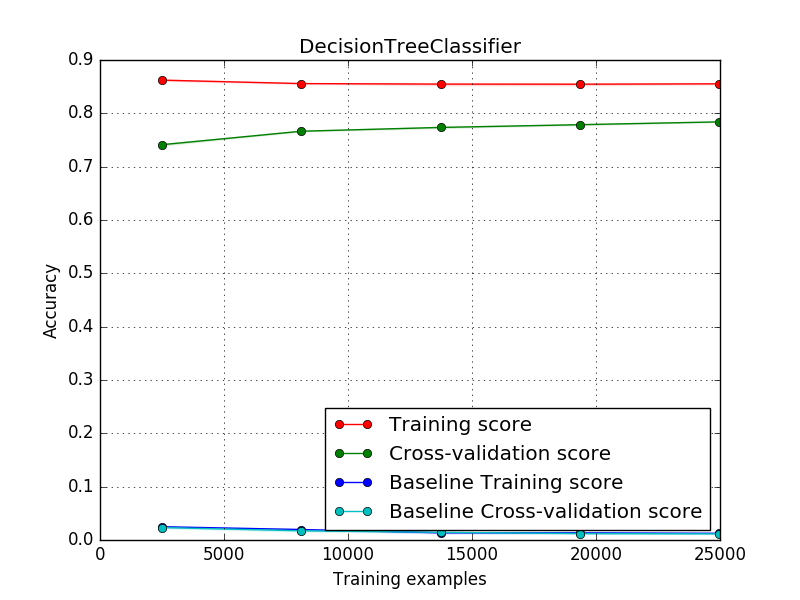
\includegraphics[width=0.6\textwidth]{Figures/Plot_DecisionTreeClassifier}
\decoRule
\caption[Learning Curve for Decision Tree Classifier]{Learning Curve for Decision Tree Classifier}
\label{fig:tree}
\end{figure}

\noindent Table~\ref{tab:tree:ctu} shows the results from the experiments that were done on the CTU-dataset. It also shows the comparison between the different feature sets. The F-score for multi-class classification is lower than the F-score from KNN. The fact that this score is lower could be due to the same reason as to why Decision tree classifiers didn't seem to be a promising algorithm. The tree is constructed using "decisions". These "decisions" could be too simple to be able to accurately define a specific class. \\
\\
However, the high binary F-score shows that even though the decisions might not always lead to the correct classification, they do lead to the correct decision of being malicious or non-malicious. The variance on the results is very small which means that the algorithm is stable and produces statistically relevant results. \\
\\
The different features perform is a similar way as they performed for KNN. Using the TCP flags increases the F-scores of the algorithm. This means that somewhere in the tree, a decision is made using these TCP flags and that this decision does help with correctly classifying the samples. The country feature set does not increment the performance. The results between the country feature set and the standard feature set only differ with just a few samples. The decision tree classifier is not able to use the country of origin at all. This does seem to follow the assumption that the dataset just does not contain enough different countries to allow the algorithm to make any decisions.

\begin{table}[H]
\caption{Decision Tree Classifier: comparing different feature sets: CTU-dataset}
\label{tab:tree:ctu}
\centering
\begin{tabular}{l c c r}
\toprule
Feature set & Standard & TCP & Country \\
\midrule
Multi-class F-score & 0.6001 & 0.6650 & 0.5999 \\
Multi-class Precision & 0.6571 & 0.7099 & 0.6570 \\
Multi-class Recall & 0.6008 & 0.6733 & 0.6007 \\
\midrule
Binary F-score & 0.9074 & 0.9511 & 0.9072 \\
Binary Precision & 0.8392 & 0.9175 & 0.8390 \\
Binary Recall & 0.9875 & 0.9873 & 0.9875 \\
\midrule
Total amount of samples & 195519.0 & 195519.0 & 195519.0 \\
False negative & 708.9  &  722.5 & 710.5 \\
False positive & 10762.7 & 5050.6 & 10778.9 \\
True negative & 127865.3 & 133577.4 & 127849.1  \\
True positive & 56182.1 & 56168.5  & 56180.5 \\
\midrule
Positive training samples & 25195.0 & 25195.0 & 25195.0\\
Negative training samples & 24806.0 & 24806.0 & 24806.0\\
\midrule
Variance Multi-class F-score & 1.44e-07 & 1.58e-07 & 2.44e-07 \\
Variance Multi-class Precision & 1.85e-07  &  1.92e-07 &  1.73e-07 \\
Variance Multi-class Recall &  1.76e-07 & 1.79e-07 &  2.59e-07  \\
\midrule
Variance Binary F-score & 2.92e-07  & 4.70e-08 & 5.80e-07  \\
Variance Binary Precision & 8.42e-07  &  9.15e-08  & 1.74e-06   \\
Variance Binary Recall & 8.92e-10 &  1.15e-07 & 1.56e-09 \\
\bottomrule
\end{tabular}
\end{table}

\noindent The results in Table~\ref{tab:tree:cross}, show the results of the cross-dataset evaluation which is used to evaluate the third step. Training is done using $19861$ non-malicious samples, $15000$ samples from the SQl dataset and $15000$ samples from the CTU dataset. The F-scores are higher than the F-scores from the CTU experiments. This means that the samples from the SQL dataset are more distinct and more easy to classify. It also means that the decision tree classifier is still able to correctly predict samples even though it is trained with multiple datasets. 

\begin{table}[H]
\caption{Decision Tree Classifier: comparing different feature sets: Cross-dataset}
\label{tab:tree:cross}
\centering
\begin{tabular}{l c c r}
\toprule
Feature set & Standard & TCP & Country \\
\midrule
Multi-class F-score & 0.7509 & 0.8042 & 0.7500 \\
Multi-class Precision & 0.7895 & 0.8307 & 0.7900 \\
Multi-class Recall & 0.7452 & 0.8057 & 0.7500 \\
\midrule
Binary F-score & 0.9413 & 0.9716 & 0.9400 \\
Binary Precision & 0.8946 & 0.9506 & 0.8900 \\
Binary Recall & 0.9932 & 0.9935 & 0.9900 \\
\midrule
Total amount of samples & 246467.0 & 246467.0 & 246467.0 \\
False negative & 729.7  &  700.9 & 723.9 \\
False positive & 12615.9 & 5567.7 & 12619.1 \\
True negative & 126012.1 &  133060.3 & 126008.9  \\
True positive & 107109.3 & 107138.1 & 107115.1 \\
\midrule
Positive training samples & 30140.0 & 30140.0 & 30140.0\\
Negative training samples & 19861.0 & 19861.0 & 19861.0\\
\midrule
Variance Multi-class F-score & 1.29e-07 & 1.93e-07 & 8.61e-08 \\
Variance Multi-class Precision & 1.98e-07  &  1.92e-07  &  1.08e-07 \\
Variance Multi-class Recall &  1.48e-07 &  3.21e-07 &  1.15e-07  \\
\midrule
Variance Binary F-score & 7.93e-08  & 2.05e-07 & 9.44e-08   \\
Variance Binary Precision & 2.56e-07  &  2.59e-07  & 3.19e-07    \\
Variance Binary Recall & 6.43e-09 &  2.50e-07  & 4.49e-09 \\
\bottomrule
\end{tabular}
\end{table}

\noindent As a final step, Decision tree classifiers were evaluated using a real-life unlabeled dataset. This was done using the Cegeka and EDM dataset. In Table~\ref{tab:knn:cegeka}, the results can be seen. The algorithm was tested on $\sim11000000$ samples. From these samples $10000$ were from the EDM dataset. The others are from the Cegeka dataset. Surprisingly,  the algorithm generated a huge amount of false positives. This caused to algorithm to have a really low F-score. Every sample from the EDM dataset was classified as malicious, while only $3$ actually were. The reason that Decsion tree classifiers do not work well on real-world unlabeled data is probably because it is too fixated on the training data. The other evaluation tests got good results since the algorithm could work well on data that belonged to the same dataset. The decisions that the Decision tree classifier makes expect to be fed data that is very similar as the training dataset. This was the case for the other evaluation data, but not for the data from Cegeka and EDM. 

\begin{table}[H]
\caption{Decision tree classifiers: real-world data}
\label{tab:tree:cegeka}
\centering
\begin{tabular}{l  r}
\toprule
F-score & 0.0155\\
\midrule
Total amount of samples & 11072646 \\
False negative & 14280  \\
False positive & 3245349 \\
True negative & 7787297 \\
True positive & 25720  \\
\bottomrule
\end{tabular}
\end{table}



\newpage
\section{Naive Bayes}

Naive Bayes has been explained in Section~\ref{bayesalg}. The algorithm uses the Theorem of Bayes. Not every feature is independent, for example it could be that the source and destination port are connected. Due to this reason, the algorithm was not that promising. This also showed during the experiments. \\
\\
The first experiment created the learning curve as seen in Figure~\ref{fig:naiveBayes}. In the beginning, with just a few samples, the accuracy is higher than when more training samples are used. This is due to the distribution of labels. Some labels appear more than others. When only 500 samples are used for training, most of these samples belong to classes that appear the most. Due to the fact that there are not many training samples, the algorithm has a higher chance of only predicting the most popular classes. The distribution of labels is similar when more training samples are used, but due to the higher amount of training samples, the algorithm trains more, and accounts for more labels.\\
\\
It can also be seen that both the training score and cross-validation score converge very fast. This signifies high bias and means that there is no point in training with more samples. 
 \begin{figure}[H]
\centering
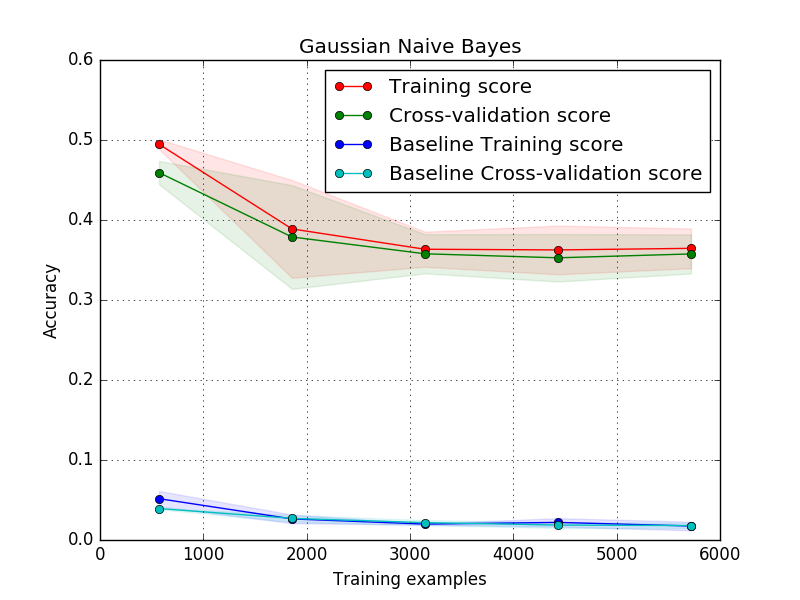
\includegraphics[width=0.6\textwidth]{Figures/Gaussian_Naive_Bayes}
\decoRule
\caption[Learning Curve for Gaussian Naive Bayes]{Learning Curve for Gaussian Naive Bayes}
\label{fig:naiveBayes}
\end{figure}

\noindent In Table~\ref{tab:bay:ctu}, the results from the CTU experiments can be seen. Immediatly two things can be seen. The scores are very low. The binary F-score is even lower than the F-score from the first baseline. The feature sets also have nearly no effect on the F-scores. The variance is also extremely small, which means these results are statistically relevant. This means that the Naive Bayes algorithm does not perform well at all. The fact that the feature sets have no effect can be contributed to the Naive assumption that is made. 	\\
\\
If the features are dependent on eachother, then the Naive assumption is completely wrong. The features extracted from flows are dependent on eachother. This can be due to the fact that packets on a network are always structured. An example would be that when the destination port is $80$, it can be expected that the protocol used is TCP. This signifies a dependence. 

\begin{table}[H]
\caption{Gaussian Naive Bayes: comparing different feature sets: CTU-dataset}
\label{tab:bay:ctu}
\centering
\begin{tabular}{l c c r}
\toprule
Feature set & Standard & TCP & Country \\
\midrule
Multi-class F-score & 0.3253 & 0.3253 & 0.3253 \\
Multi-class Precision & 0.2980 & 0.2980 & 0.2980 \\
Multi-class Recall & 0.4231 & 0.4232 & 0.4232 \\
\midrule
Binary F-score & 0.0146 & 0.0147 & 0.0147 \\
Binary Precision & 0.0179 & 0.0179 & 0.0179 \\
Binary Recall & 0.0123 & 0.0124 & 0.0124 \\
\midrule
Total amount of samples & 195519.0 & 195519.0 & 195519.0 \\
False negative & 56191.2  & 56186.0 & 56186.0 \\
False positive & 38393.0 & 38495.0 & 38495.0 \\
True negative & 100235.0 & 100133.0 & 100133.0 \\
True positive & 699.8 & 705.0 & 705.0 \\
\midrule
Positive training samples & 3545.0 & 3545.0 & 3545.0\\
Negative training samples & 4956.0 & 4956.0 & 4956.0\\
\midrule
Variance Multi-class F-score & 3.08e-33 & 3.08e-33 & 3.08e-33 \\
Variance Multi-class Precision & 0.0 &  0.0 & 0.0\\
Variance Multi-class Recall &  0.0 & 0.0 &  0.0   \\
\midrule
Variance Binary F-score & 0.0 &  0.0  & 0.0 \\
Variance Binary Precision & 1.20e-35 &  1.20e-35 & 1.20e-35  \\
Variance Binary Recall & 0.0 & 0.0 & 0.0 \\
\bottomrule
\end{tabular}
\end{table}

\noindent During the cross-dataset validation in Table~\ref{tab:bay:cross}, similar results can be seen. It can be noted that the binary F-score is higher and barely above the binary F-score from the first baseline. This means that even if the features are not independent, the algorithm can still see differences between SSH scans and normal traffic. Due to the fact that Bayes does not perform well at all, it has not been used in step four.

\begin{table}[H]
\caption{Gaussian Naive Bayes: comparing different feature sets: Cross-dataset}
\label{tab:bay:cross}
\centering
\begin{tabular}{l c c r}
\toprule
Feature set & Standard & TCP & Country \\
\midrule
Multi-class F-score & 0.3403 & 0.3398 & 0.3398 \\
Multi-class Precision & 0.3175 & 0.3170 & 0.3170 \\
Multi-class Recall & 0.4052 & 0.4047 & 0.4047 \\
\midrule
Binary F-score & 0.4990 & 0.4988 & 0.4986 \\
Binary Precision & 0.4854 & 0.4847 & 0.4843 \\
Binary Recall & 0.5134 & 0.5136 & 0.5137 \\
\midrule
Total amount of samples & 246467.0 & 246467.0 & 246467.0 \\
False negative & 52474.5  &  52452.9 & 52474.5 \\
False positive & 58695.1 & 58882.7 & 58695.1 \\
True negative & 79932.9 & 79745.3 & 79932.9  \\
True positive & 55364.5 & 55386.1 & 55364.5 \\
\midrule
Positive training samples & 6545.0 & 6545.0 & 6545.0\\
Negative training samples & 4956.0 & 4956.0 & 4956.0\\
\midrule
Variance Multi-class F-score & 3.26e-06 & 4.07e-06 & 4.92e-06\\
Variance Multi-class Precision & 3.31e-06 &  3.80e-06 & 4.52e-06 \\
Variance Multi-class Recall &  2.72e-06 & 3.90e-06 &  3.95e-06   \\
\midrule
Variance Binary F-score & 1.15e-06 & 1.31e-06 & 1.26e-06 \\
Variance Binary Precision & 5.09e-06 &  5.05e-06  & 3.07e-06   \\
Variance Binary Recall & 1.22e-06 &  8.18e-07 & 9.2e-07 \\
\bottomrule
\end{tabular}
\end{table}

\newpage
\section{Support Vector machines with Linear Kernel}

Support Vector Machines have also been tested. These have been explained in Section~\ref{svmalg}. First Support Vector Machines with a linear kernel have been tested. In the next section, Support Vector Machines with an RBF kernel has been used. \\
\\
The learning curve, shown in Figure~\ref{fig:svml}, is very irregular. It does not seem to follow a pattern at all. There is also a big standard deviation on the results. The accuracy almost matches the baseline in the worst case. Due to the irregular nature, it could lead to the conclusion that overfitting occurs since the cross-validation score drops. However, the training score also drops, which is not expected during overfitting. Underfitting could occur, but in that case it would be expected to see a slight increase in the accuracy instead on the extreme variance. 

 \begin{figure}[H]
\centering
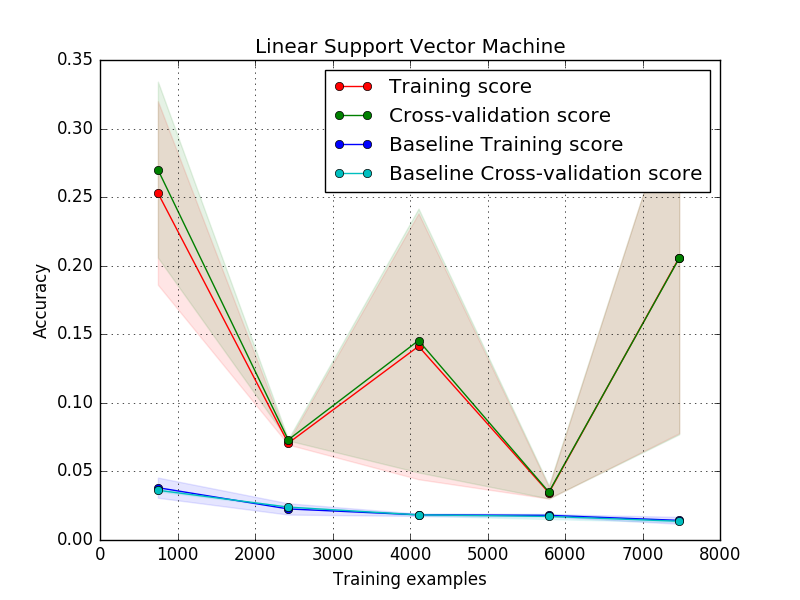
\includegraphics[width=0.6\textwidth]{Figures/Linear_Support_Vector_Machine}
\decoRule
\caption[Learning Curve for Linear Support Vector Machine]{Learning Curve for Linear Support Vector Machine}
\label{fig:svml}
\end{figure}

\noindent In Table~\ref{tab:linsvm:ctu}, the results from the experiments using the CTU dataset are shown. The first element that can be seen is the high variance. These mean that it becomes difficult to compare the results from the different feature sets. Furthermore, the F-scores are barely equal to the F-scores from the baseline. \\
\\
These scores and the variance can be explained due to the fact that intrusion detection cannot be solved using a linear classifier. Since there are a lot of features, it is difficult to plot them, so Figure~\ref{fig:linearvsNonLinearClassifier} from Section~\ref{linearclass} will be used. The linear classifier cannot group the different classes together. Every group created by the linear classifier still contains a lot of samples from other classes. This explains the low F-scores. With multi-class classification, a different linear classifier is used for each class. A linear classifier cannot find a good way to divide samples belonging to a class, and not belonging to the class. In total, there are over a hunderd classes. Each time the experiment is done, the linear classifier for each class is slightly different since it cannot find a way to correctly group each class. This slight difference adds up for a hunderd classes and causes the high variance on the F-scores. 

\begin{table}[H]
\caption{Linear Kernel Support Vector Machine: comparing different feature sets: CTU-dataset}
\label{tab:linsvm:ctu}
\centering
\begin{tabular}{l c c r}
\toprule
Feature set & Standard & TCP & Country \\
\midrule
Multi-class F-score & 0.1015 & 0.0191 & 0.1883 \\
Multi-class Precision & 0.2091 & 0.0437 & 0.3218 \\
Multi-class Recall & 0.0918 & 0.0330 & 0.1621 \\
\midrule
Binary F-score & 0.4159 & 0.2267 & 0.4158 \\
Binary Precision & 0.2890 & 0.1470 & 0.2842 \\
Binary Recall & 0.7914 & 0.5007 & 0.7935 \\
\midrule
Total amount of samples & 195519.0 & 195519.0 & 195519.0 \\
False negative & 11866.5 & 28402.9 & 11747.6 \\
False positive & 90404.1 & 76436.5 & 87959.7 \\
True negative & 48223.9 & 62191.5 & 50668.3 \\
True positive & 45024.5 & 28488.1 & 45143.4 \\
\midrule
Positive training samples & 10069.0 & 10069.0 & 10069.0\\
Negative training samples & 9932.0 & 9932.0 & 9932.0\\
\midrule
Variance Multi-class F-score & 0.02 & 0.05 & 0.02020\\
Variance Multi-class Precision & 0.03 &  0.02 & 0.0279\\
Variance Multi-class Recall &  0.02 & 0.0001 &  0.0189   \\
\midrule
Variance Binary F-score & 0.05 &  0.05  & 0.0464 \\
Variance Binary Precision & 0.03 &  0.02 & 0.0233 \\
Variance Binary Recall & 0.15 & 0.25 & 0.1574 \\
\bottomrule
\end{tabular}
\end{table}

\noindent The cross-dataset experiments shown in Table~\ref{tab:linsvm:cross} have a lower variance. However, compared to other algorithms, the variance is still very high. The F-scores are overall a bit higher than the F-scores from the baseline, which means that the F-scores are not great at all. The results from this experiment are similar to the CTU experiment and the explanation of why the algorithm does not perform well is still supported due to the low scores and the high variance. Due to the fact that Support Vector Machines using a linear kernel do not perform well at all, it has not been used in step four.

\begin{table}[H]
\caption{Linear Kernel Support Vector Machine: comparing different feature sets: Cross-dataset}
\label{tab:linsvm:cross}
\centering
\begin{tabular}{l c c r}
\toprule
Feature set & Standard & TCP & Country \\
\midrule
Multi-class F-score & 0.2009 & 0.0369 & 0.2095 \\
Multi-class Precision & 0.3925 & 0.0533 & 0.4191 \\
Multi-class Recall & 0.1478 & 0.0497 & 0.1556 \\
\midrule
Binary F-score & 0.6041 & 0.4974 & 0.6390 \\
Binary Precision & 0.4952 & 0.4263 & 0.4703 \\
Binary Recall & 0.9183 & 0.6796 & 0.9971 \\
\midrule
Total amount of samples & 246467.0 & 246467.0 & 246467.0 \\
False negative & 8806.2  & 34551.5 & 314.2\\
False positive & 112296.5 & 89987.9 & 121331.3 \\
True negative & 26331.5 & 48640.1 & 517296.7 \\
True positive & 99032.8 & 73287.5 & 107524.8 \\
\midrule
Positive training samples & 10045.0 & 10045.0 & 10045.0\\
Negative training samples & 4956.0 & 4956.0 & 4956.0\\
\midrule
Variance Multi-class F-score & 0.0023 & 0.0027 & 0.0009\\
Variance Multi-class Precision & 0.0041 &  0.0053 & 0.0004\\
Variance Multi-class Recall &  0.0022 & 0.0049 &  0.0009   \\
\midrule
Variance Binary F-score & 0.0084 &  0.0309  & 0.0001 \\
Variance Binary Precision & 0.0084 &  0.0240 & 0.0002 \\
Variance Binary Recall & 0.0551 & 0.1003 & 1.1332e-06 \\
\bottomrule
\end{tabular}
\end{table}

\newpage
\section{Support Vector machines with RBF Kernel}

Support Vector Machines using a linear kernel did not work at all. They were barely better than the baseline. A conclusion was made that the classification cannot be made using linear classification. This can be verified by using a non-linear kernel. The kernel that was used, is the RBF kernel as seen in Section~\ref{kernels}. \\
\\
The learning curve is shown in Figure~\ref{fig:svmlearn}. Immediatly can be seen that the learning curve looks much better. The curve is regular. In this learning curve, it can be seen that there is a big gap between the cross-validation and training score. In underfitting, both the training and cross-validation score should be low. This cannot be seen in this learning curve. During overfitting, it would be expected that the training score is high since the model fits the training data very well, however the cross-validation score should be low and dropping. However, this also cannot be seen in this learning curve.

 \begin{figure}[H]
\centering
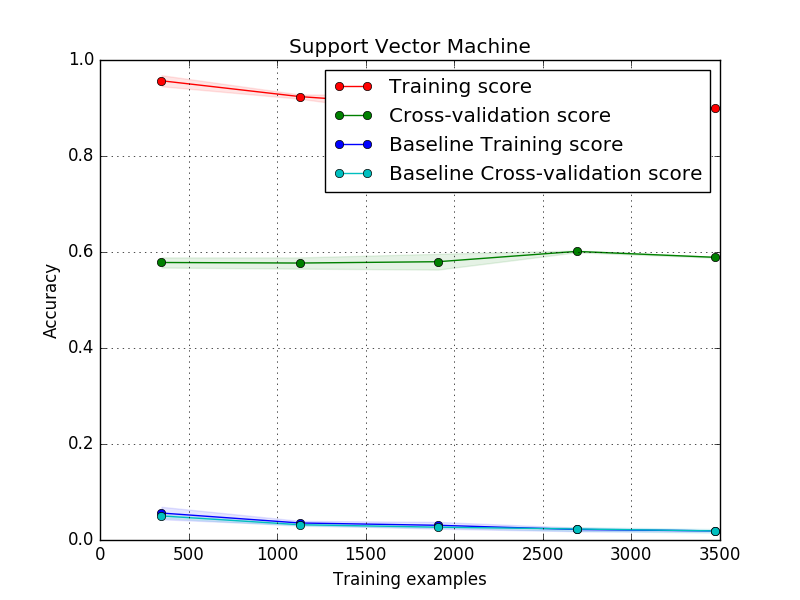
\includegraphics[width=0.6\textwidth]{Figures/Support_Vector_Machine}
\decoRule
\caption[Learning Curve for Support Vector Machine]{Learning Curve for Support Vector Machine}
\label{fig:svmlearn}
\end{figure}

\noindent The results from the CTU experiments are shown in Table~\ref{tab:svm:ctu}. The variance on both F-scores are very low which means we can compare the different F-scores. The multi-class F-scores are higher than the multi-class F-scores from the experiments with the linear kernel. This means that the exact classification happens better when using a non-linear kernel. This supports the idea that the classification cannot happen with a linear classifier. \\
\\
However, the binary F-score is extremely low. This is a result from using the RBF kernel. RBF kernels are also called Gaussian kernels. The kernel expects that training data follows a Gaussian distribution which is not the case for the training data from intrusion detection. The malicious and non-malicious samples do not follow a Gaussian distribution at all. When trying to classify samples using a Gaussian distribution, it cannot see the difference between malicious or non-malicious. More concretely, it seems that the algorithm cannot detect malicious samples at all. It classifies most samples as non-malicious. However, it can still see the difference between some non-malicious classes. Because of that the multi-class F-score seems to be higher. \\
Even though the binary F-score is much lower than the binary F-score from the experiments with linear kernels, both are worse than the baseline.The results from the multi-class F-score can also be compared to the multi-class F-score from the linear kernels. The multi-class F-score is still much higher than the multi-class F-score from the baseline. This means that the algorithm can still classify results better than randomly. The different feature sets also have little to no effect on the F-score, in case of the TCP feature set, it even lowers the F-score. 

\begin{table}[H]
\caption{RBF Kernel Support Vector Machine: comparing different feature sets: CTU-dataset}
\label{tab:svm:ctu}
\centering
\begin{tabular}{l c c r}
\toprule
Feature set & Standard & TCP & Country \\
\midrule
Multi-class F-score & 0.3641 & 0.3030 & 0.3643 \\
Multi-class Precision & 0.5124 & 0.5554 & 0.5167 \\
Multi-class Recall & 0.4037 & 0.3589 & 0.4062 \\
\midrule
Binary F-score & 0.0455 & 0.0282 & 0.0449 \\
Binary Precision & 0.0749 & 0.9987 & 0.0758 \\
Binary Recall & 0.0327 & 0.0143 & 0.0319 \\
\midrule
Total amount of samples & 195519.0 & 195519.0 & 195519.0 \\
False negative & 55029.0 & 56077.5 & 55075.0 \\
False positive & 22991.0 & 1.0 & 22115.0 \\
True negative & 115637.0 & 138627.0 & 116513.0 \\
True positive & 1862.0 & 813.5 & 1816.0\\
\midrule
Positive training samples & 2522.0 & 2522.0 & 2522.0\\
Negative training samples & 2479.0 & 2479.0 & 2479.0\\
\midrule
Variance Multi-class F-score & 3.08e-33 & 0.0 & 3.08e-33 \\
Variance Multi-class Precision & 0.0 & 1.23e-32 & 1.23e-32 \\
Variance Multi-class Recall & 1.23e-32 & 0.0 & 3.08e-33  \\
\midrule
Variance Binary F-score & 0.0 & 1.20e-35 & 4.81e-35 \\
Variance Binary Precision & 0.0 & 1.23e-32 & 0.0 \\
Variance Binary Recall & 4.81e-35 & 0.0 & 4.81e-35 \\
\bottomrule
\end{tabular}
\end{table}

\noindent The results from the cross-dataset validation are shown in Table~\ref{tab:svm:cross}. These results are much better. It seems that the SSH scans can
be detected better than the malware from the CTU dataset. The effect of using the TCP feature set and Country feature set is quite significant. This means that these feature do help the algorithm to correctly classifiy samples. However, this seems to only be the case for the SSH scans, not the samples from the CTU dataset. \\
\\
This can have two explanations. The first explanation is that using the TCP flags that are used allow the SVM to make a distinction between samples from the SQL dataset and the CTU dataset. This means that during predictions, it can also distinguish between samples from the SQL dataset and the CTU dataset. In other words, the algorithm is affected by the origin of the data. \\
\\
The other explanation is that the distinction between SSH scans and normal behaviour is quite large when the TCP flags are used, but malware and normal behaviour still look the same to the SVM.  This means that the SVM can see differences between some classes, but not between all classes. Since such a difference between CTU datasets and Cross-dataset experiments can only be seen in experiments using SVM with a RBF kernel, it seems that the second explanation is more plausible. Due to the fact that Support Vector Machines using a RBF kernel do not perform well at all, it has not been used in step four.

\begin{table}[H]
\caption{RBF Kernel Support Vector Machine: comparing different feature sets: Cross-dataset}
\label{tab:svm:cross}
\centering
\begin{tabular}{l c c r}
\toprule
Feature set & Standard & TCP & Country \\
\midrule
Multi-class F-score & 0.3352 & 0.5761 & 0.5764 \\
Multi-class Precision & 0.6524 & 0.6944 & 0.6982 \\
Multi-class Recall & 0.4277 & 0.5979 & 0.5997 \\
\midrule
Binary F-score & 0.6740 & 0.6974 & 0.7001 \\
Binary Precision & 0.5083 & 0.7492 & 0.7567 \\
Binary Recall & 0.9999 & 0.6524 & 0.6514 \\
\midrule
Total amount of samples & 246467.0 & 246467.0 & 246467.0 \\
False negative & 10.8 & 37484.0 & 37584.4 \\
False positive & 104306.8 & 23541.0 & 22587.7 \\
True negative & 34321.2 & 115087.0 & 116040.3 \\
True positive & 107828.2 & 70355.0 & 70254.6 \\
\midrule
Positive training samples & 4522.0 & 4522.0 & 4522.0\\
Negative training samples & 2479.0 & 2479.0 & 2479.0\\
\midrule
Variance Multi-class F-score & 4.46e-08 & 3.92e-08 & 2.64e-07\\
Variance Multi-class Precision & 6.53e-06 & 3.30e-08 & 8.75e-08 \\
Variance Multi-class Recall & 2.16e-08 & 1.00e-07 & 6.01e-07  \\
\midrule
Variance Binary F-score & 5.71e-09 &  2.65e-07 & 1.42e-06\\
Variance Binary Precision & 6.50e-09 & 8.58e-08 & 1.96e-07 \\
Variance Binary Recall & 5.50e-09  & 4.76e-07 & 3.0685e-06 \\
\bottomrule
\end{tabular}
\end{table}

\newpage
\section{Neural network}

Neural networks were a promising algorithm. They were explained in Section~\ref{neuralnet}. Neural networks are quite complex and contain a lot of weights that need to be calculated during the training phase. Because of this, they require to be trained using a lot of data or they can be unstable and be in an underfitting phase. \\
\\
The learning curve can be seen in Figure~\ref{fig:neural}. The first thing that can be seen is that the training score and the cross-validation score are very close together. The scores are also dropping. Neural network requires a lot of training data. However, in the available datasets there is only a couple of thousand samples per malicious classification. The accuracy keeps dropping. This does not signify overfitting as the training score is also low. However, it does seem to be related to underfitting. During underfitting, it is expected that the training and cross-validation score drop to a local minimum and afterwards starts increases as the overfitting is resolved. However, there is not enough data to test when the overfitting is resolved.

 \begin{figure}[H]
\centering
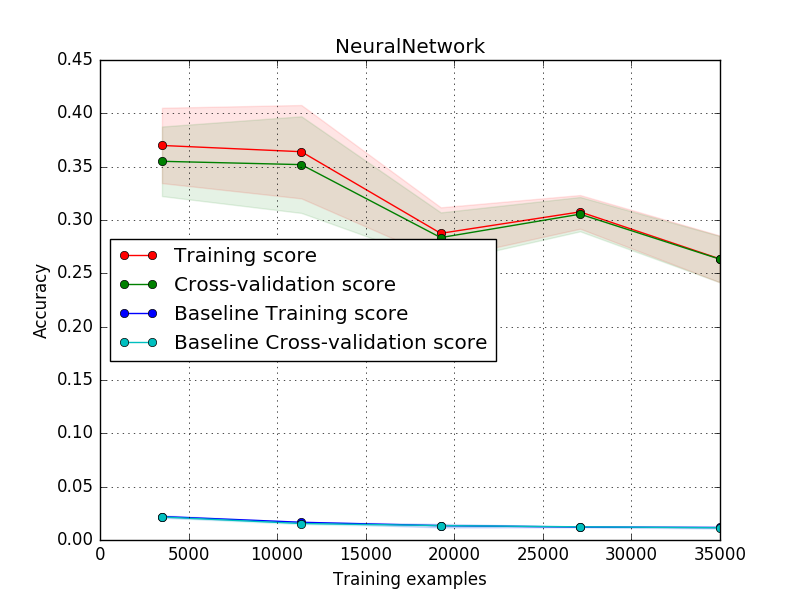
\includegraphics[width=0.6\textwidth]{Figures/NeuralNetwork}
\decoRule
\caption[Learning Curve for Neural Network]{Learning Curve for Neural Network}
\label{fig:neural}
\end{figure}

\noindent Even though the algorithm underfits, the experiments were still done. The results from the CTU dataset are shown in Table~\ref{tab:neural:ctu}. The Binary F-score is $0$ which means that the algorithm always classifies samples as non-malicious. The multi-class F-score is also quite low. This could be contributed to the underfitting. \\
\\
The biggest piece of evidence is the F-scores for the different feature sets. The multi-class F-scores for the TCP feature set and the Country feature set are much lower. These feature sets contain more features compared to the standard feature set. In a neural network, this means that more weights need to be calculated. This means that the overfitting should be worse when using more features. This is reflected in the F-scores for the TCP and Country feature set.

\begin{table}[H]
\caption{Neural Network: comparing different feature sets: CTU-dataset}
\label{tab:neural:ctu}
\centering
\begin{tabular}{l c c r}
\toprule
Feature set & Standard & TCP & Country \\
\midrule
Multi-class F-score & 0.2213 & 0.1322 & 0.1763 \\
Multi-class Precision & 0.2070 & 0.0854 & 0.1479 \\
Multi-class Recall & 0.3541 & 0.2922 & 0.3225 \\
\midrule
Binary F-score & 0.0 & 0.0 & 0.0 \\
Binary Precision & 0.0 & 0.0 & 0.0 \\
Binary Recall & 0.0 & 0.0 & 0.0 \\
\midrule
Total amount of samples & 195519.0 & 195519.0 & 195519.0 \\
False negative & 56891.0 & 56891.0 & 56891.0 \\
False positive & 0.0 & 0.0 & 0.0 \\
True negative & 138628.0 & 138628.0 & 138628.0 \\
True positive & 0.0 & 0.0 & 0.0 \\
\midrule
Positive training samples & 25195.0 & 25195.0 & 25195.0\\
Negative training samples & 24806.0 & 24806.0 & 24806.0\\
\midrule
Variance Multi-class F-score & 0.0019 & 7.70e-34 & 0.0029 \\
Variance Multi-class Precision & 0.0037 & 0.0 & 0.0059 \\
Variance Multi-class Recall & 0.0009 & 0.0 & 0.0013  \\
\midrule
Variance Binary F-score & 0.0 & 0.0 & 0.0 \\
Variance Binary Precision & 0.0 & 0.0 & 0.0 \\
Variance Binary Recall & 0.0 & 0.0 & 0.0 \\
\bottomrule
\end{tabular}
\end{table}

\noindent The results from the cross-dataset validation is shown in Table~\ref{tab:neural:cross}. The scores are yet again, quite low. The algorithm was trained using $20000$ samples from the SQL dataset, $25000$ malicious samples from the CTU dataset and $25000$ non-malicious samples from the CTU dataset. \\
\\
The binary F-score is much higher as compared to the CTU experiment. It has to be noted that the samples of the SQL dataset belong to a single class, SSH scans and that the malicious samples from the CTU dataset contain a lot of different malicious classes. This means that if the binary F-score is higher, the neural net does not underfit that much anymore on the classification between malicious and non-malicious. This is due to the SSH scan samples. This leads to the conclusion that the algorithm is should not underfit that much anymore when more than $20000$ samples are used for each class. \\
\\
It is also interesting that the multi-class F-score for the TCP feature set is much higher as compared to the other multi-class F-scores. This is also due to the samples from the SQL dataset. It seems that having these samples does indeed resolve a part of the underfitting, especially when the TCP flags are used. Even though more weights need to be calculated, it seems that the TCP flags help more than they cause underfitting. Due to the fact that Neural networks do not perform well and are underfitting, it has not been used in step four. 

\begin{table}[H]
\caption{Neural Network: comparing different feature sets: Cross-dataset}
\label{tab:neural:cross}
\centering
\begin{tabular}{l c c r}
\toprule
Feature set & Standard & TCP & Country \\
\midrule
Multi-class F-score & 0.1338 & 0.3679 & 0.1433 \\
Multi-class Precision & 0.0908 & 0.3328 & 0.0968 \\
Multi-class Recall & 0.2901 & 0.5021 & 0.2986 \\
\midrule
Binary F-score & 0.6128 & 0.5514 & 0.6056 \\
Binary Precision & 0.4426 & 0.5507 & 0.4437 \\
Binary Recall & 0.9970 & 0.5635 & 0.9641 \\
\midrule
Total amount of samples & 246467.0 & 246467.0 & 246467.0 \\
False negative & 316.9 & 47071.7 & 3867.5 \\
False positive & 135732.8 & 49578.2 & 130776.2 \\
True negative & 2895.2 & 89049.8 & 7851.8 \\
True positive & 107522.1 & 60767.3 & 103971.5 \\
\midrule
Positive training samples & 45195.0 & 45195.0 & 45195.0\\
Negative training samples & 24806.0 & 24806.0 & 24806.0\\
\midrule
Variance Multi-class F-score & 0.0006 & 0.0019 & 0.0013 \\
Variance Multi-class Precision & 0.0009 & 0.0028 & 0.0010 \\
Variance Multi-class Recall & 0.0003 & 0.0017 & 0.0009  \\
\midrule
Variance Binary F-score & 0.0001 & 0.0024 & 0.0006 \\
Variance Binary Precision & 0.0002 & 0.0039 & 0.0002 \\
Variance Binary Recall & 7.77e-05 & 0.0075 & 0.009 \\
\bottomrule
\end{tabular}
\end{table}

\newpage
\section{One-class Support Vector Machines}
\label{eval:oneclass}
One-class Support Vector Machines are the only unsupervised learning algorithms that have been used. They are explained in Section~\ref{oneclassSVM}. One-class Support Vector Machines only use a single class. The idea behind the algorithm was to perhaps use it as a preprocessor. If the algorithm would be able to correctly predict whether an element is malicious or non-malicious, it could be used before a supervised algorithm would be used. Afterwards, only the malicious samples would be fed to a supervised learning algorithm.\\
\\
Table~\ref{tab:one:cross} shows the results from different experiments that have been done. Yet again, it can be seen that using the TCP feature set does increase the performance. However, even with the TCP feature set, the binary F-score is barely as good as the baseline, a random classifier. Looking more closely, it can be seen that there are no true negatives in the TCP feature set experiment. However, there are false negatives. This means that the algorithm cannot be used at all for a preprocessing step. \\
\\
As said before, one-class Support Vector Machine uses only a single class. Once they are trained, they can predict whether an element belongs to this class or not. This class is made by using a RBF kernel. The results show that the SVM cannot properly define the boundaries of the class. This means that there are a lot of samples that are predicted wrong. Using the TCP flags probably make the class boundary even more irregular as compared to using the standard feature set. This means that the class becomes so large that almost every possible sample becomes part of the class. This causes the effect that even the non-malicious samples are all predicted to be malicious.  This effect is not seen in the country feature set. That can be explained by the fact that in the country feature set, the IP address features are replaced by the country of origin. This has the effect that the class is defined more or less the same. 

\begin{table}[H]
\caption{One-class Support Vector Machine: comparing different feature sets: Cross-dataset}
\label{tab:one:cross}
\centering
\begin{tabular}{l c c r}
\toprule
Feature set & Standard & TCP & Country \\
\midrule
Binary F-score & 0.1275 & 0.4017 & 0.1557\\
Binary Precision & 0.1128 & 0.2911 & 0.1385 \\
Binary Recall & 0.1489 & 0.6480 & 0.1794\\
\midrule
Total amount of samples & 226467.0 & 226467.0 & 226467.0 \\
False negative & 74762.4 & 30912.0 & 72082.7 \\
False positive & 88162.5 & 138628.0 & 87260.7 \\
True negative & 50465.6 & 0.0 & 51367.3 \\
True positive & 13076.5 & 56927.0 & 15756.3 \\
\midrule
Positive training samples & 65000.0 & 65000.0 & 65000.0\\
Negative training samples & 0.0 & 0.0 & 0.0\\
\midrule
Variance Binary F-score & 0.0191 & 0.0006 & 0.0169 \\
Variance Binary Precision & 0.0125 &  0.0002 & 0.0116 \\
Variance Binary Recall & 0.0319 & 0.0024 & 0.0261 \\
\bottomrule
\end{tabular}
\end{table}

% Chapter Template

\chapter{Future work} % Main chapter title

\label{prevention} % Change X to a consecutive number; for referencing this chapter elsewhere, use \ref{ChapterX}

\section{Prevention}
This chapter will only be done if this is made in the thesis
\subsection{Real-time detection}

\subsection{Data limiting}

\subsection{Connection closing}

% Chapter Template

\chapter{Conclusion} % Main chapter title

\label{conclusion} % Change X to a consecutive number; for referencing this chapter elsewhere, use \ref{ChapterX}


%----------------------------------------------------------------------------------------
%	BIBLIOGRAPHY
%----------------------------------------------------------------------------------------

\printbibliography[heading=bibintoc]

%----------------------------------------------------------------------------------------
%	THESIS CONTENT - APPENDICES
%----------------------------------------------------------------------------------------

\appendix % Cue to tell LaTeX that the following "chapters" are Appendices

% Appendix Template

\chapter{User guide} % Main appendix title

\label{config} % Change X to a consecutive letter; for referencing this appendix elsewhere, use \ref{AppendixX}

\section{Running}
The main program can be run using the command in Listing~\ref{command}. If no config file is passed as argument the program will look for a config file named "config.json" in the current directory. \\
\begin{lstlisting}[frame=single, label=command]
python main.py [config-file-location]
\end{lstlisting}

\section{Running multiple tests}
It is also possible to run multiple tests automatically. This can be done using the command as seen in Listing~\ref{commandmult}. If no config file is passed as argument the program will look for a config file named "testing.json" in the current directory. The layout of the config file is fairly simple. It should be a list of config files that have to be run as seen in Listing~\ref{commandmultexample}. \\

\begin{lstlisting}[frame=single, label=commandmult]
python testing.py [config-file-location]
\end{lstlisting}

\begin{lstlisting}[language=json,firstnumber=1, label=commandmultexample]
[
    "main/config.json"
]
\end{lstlisting}

\section{Config file}
The config file contains the main variables that define the execution of the program. If the format of an attribute is not correct, the program either skips that value or halts program execution. \\
\\
There are five important boolean settings in the config file. \textbf{enable-IDS} is a boolean which specifies whether the IDS should run or not. \textbf{pcap-to-flow} is whether the small, built-in flow-converter should be used. This is used to convert \textit{pcap} files to flow files. \textbf{print-labels} activates a section of the program which extracts and prints the labels that belong to a given dataset. This could be useful when trying to find out which labels the currently selected dataset will use.  \\
\\
The booleans \textbf{check} and \textbf{sniffer} can only be used when \textbf{enable-IDS} is set to \textit{True}. \textbf{check} is used to activate or disable the checking of datasets after the training phase. \textbf{sniffer} is used to activate the built-in packet sniffer. The packet sniffer sniffs packets and builts flows, which are then fed to the machine learning algorithm. \\
\begin{lstlisting}[language=json,firstnumber=1,label={configmain}]
{
    "enable-IDS" : true,
    "pcap-to-flow" : false,
    "print-labels" : false
    
    "check" : true,
    "sniffer" : false,
\end{lstlisting}~\\
\noindent \textbf{pcap-files} is a list of (source, destination) tuples for files that have to be converted using the built-in flow converter. \\

\begin{lstlisting}[language=json,firstnumber=1]
    "pcap-files" : [
        {
            "src" : "../../test/dosattack.pcap",
            "dest" :  "../../test/dosattack2.flow"
        }
    ],
\end{lstlisting}~\\
\noindent \textbf{algorithm} is used to define which algorithm is used. The value of this attribute should match the name of one of the implemented machine learning algorithm classes. \textbf{featureClass} is used to select which class to use to retrieve  features from a flow. \textbf{trainer} is used to select the training method. When the value is set to "Trainer", it is possible to select the training class in the data sets. \\

\begin{lstlisting}[language=json,firstnumber=1]
    "algorithm" : "KNeighborsClassifier",
    "featureClass" : "FlowFeature",
    "trainer" : "Trainer",
\end{lstlisting}~\\
\noindent Some attributes in the config file are used to save and use the models that the machine learning algorithms make. \textbf{model\_dir} is used to define the directory location. \textbf{model} defines the name of the model file. \textbf{use\_model} and \textbf{store\_model} are respectively used to activate usage and saving of the model. \\

\begin{lstlisting}[language=json,firstnumber=1]
    "model_dir" : "../../models/",
    "model" : "model.mdl",
    "use_model" : false,
    "store_model" : true,
\end{lstlisting}~\\
\noindent \textbf{data-sets} indicates the data to be used when training. The layout of each item in the list is dependent of which loader should be used. A netflow file has the attributes: \textbf{file}, \textbf{from} and \textbf{to}. An SQL trainer is also implemented. Here the attributes should indicate the \textbf{host}, the \textbf{user}, the \textbf{database} and the \textbf{password}. The \textbf{type} can be used to indicate which type of date it is. This should be the name of a trainer class. \\
\\
The \textbf{check-sets} are used to check the performance of the machine learning algorithm. Here the \textbf{type} indicates which type the data is. The possible values are: "file" and "sql". \\

\begin{lstlisting}[language=json,firstnumber=1]
    "data-sets" : [
            {
                "file" : "../../test/capture20110815.binetflow",
                "from" : 0,
                "to" : 40000
            },
            {
                "host" : "localhost",
                "type" : "SQLTrainer",
                "user" : "user",
                "db" : "dataset",
                "password" : "password"
            }
        ],
    

    "check-sets" : [
            {
                "file" : "../../test/capture20110815.binetflow",
                "type" : "file",
                "from" : 0,
                "to" : -1
            }
        ],
\end{lstlisting}~\\
\noindent \textbf{feature-file} is a file that can contain information to be used in the feature class. The layout of this file is dependent on which "featureClass" is used. \textbf{logger} indicates the location of the log file to use. \textbf{good-labels} indicate which labels are considered to belong to normal behaviour.

\begin{lstlisting}[language=json,firstnumber=1]
    "feature-file" : "features.json",
    "logger" : "log.txt",
    "good-labels" : "good.txt",
\end{lstlisting}~\\
\noindent The following attributes are used in the small sniffer that was implemented. \textbf{protocol-file} is a file that selects which protocols to use.  \textbf{timeout} is a value that define the amount of milliseconds to wait before closing a flow after the last packet in that flow.

\begin{lstlisting}[language=json,firstnumber=1]
    "protocol-file" : "protocols.json",
    "timeout" : 5000,
\end{lstlisting}~\\
\noindent In order to be able to test multiple algorithms at a time, there is another method next to the \textit{testing.py} file. During testing it was found that making a lot of config files was cumbersome work. A new feature was added to the config file. An attribute \textbf{configs} can be added. This should be a list. \\
\\
Each element of this list, represents a distinct config file. The variables in the "outer"/"main" config file are considered the standard values. Each element in the list can overwrite these elements. For example, below the list contains two elements which have different algorithms. The data-sets and check-sets are the same for these two "config" files. \textbf{use\_main} is used to let the program know whether to execute and "use" the outer config aswell, or to only use the configs list.
\begin{lstlisting}[language=json,firstnumber=1]
    "use_main" : true,
    "configs" : [
        {
            "algorithm" : "KNeighborsClassifier"
        },
        {
            "algorithm" : "SupportVectorMachines"
        }
    ],
}
\end{lstlisting}

% Appendix A

\chapter{Developer Guide} % Main appendix title
\label{framework}
The implementation is made to be modular. Adding new algorithms or features is as simple as adding a new class. Each module forms an important part of the implementation, such as the algorithm, the feature extraction and the data loaders.

\section{Machine learning module}
New machine learning algorithms can be added to the implementation by creating a new class and placing the class in the \textit{ml.py} file. A base class, \textbf{MLAlgorithm}, has to be inherited from and two methods have to be implemented: \\
\begin{python}
class SomeAlgorithm(MLAlgorithm):
    def train(self, data_set, target_set=None):
        data_set is an array of features
        target_set is an array of labels
            (or none for unsupervised learning)

    def predict(self, sample, corr=None):
        sample is a feature that is going 
            to be used for prediction
        corr is the correct label that 
            should be predicted
\end{python}

\section{Feature module}
A feature class is used to parse a flow. The \textbf{Flow} class is a simple "struct" like class that contains the necessary member variables for a flow. The \textbf{Flows} class is a collection of flows. To make a new featureClass, a base class, \textbf{BasicFeature}, has to be inherited from and two methods have to be implemented:\\

\begin{python}
class FlowFeature(BasicFeature):
    def __init__(self, file):
        file is a json file that may contain extra 
        information to make a featureClass 
        more reusable
        
    def make_record(self, flow):
        flow is an instance of the Flow class
        return an array of numbers to be fed 
            to a machine learning algorithm
\end{python}

\section{Loader module}
The loader module is responsible for loading the flows from any external source. The exernal source could be a text file or a SQL database. The new class should be placed in the \textit{loader.py} file. The loader class should be defined using a load and a get\_netflow method. The parameters of load can be chosen at will since the loading has to be implemented in a training class. \\
\begin{python}
class LoaderName:
    def load(self, ...):
        load the data from the source
        
    def get_netflow(self):
        return the netflow
\end{python}

\section{Prediction Module}
\noindent If a new type of loader needs to be used in the check-sets, a class has to be added to the Prediction module in the \textit{prediction\_type.py} file.  A base class, \textbf{PredictionLoader}, has to be inherited from and a method has to be implemented: "load(self, data)". "data" is a dictionary loaded from the config file.\\
\begin{python}
class PredictionFile(PredictionLoader):
    def load(self, data):
        return the netflow
\end{python}

\section{Training module}
The training module is responsible for all training classes. New types of training can be added to the implementation by creating a new class and placing the class in the \textit{train.py} file. A base class, \textbf{Trainer}, has to be inherited from and a method has to be implemented. The method has several parameters. "algorithm" is an instance of a machine learning algorithm. "data" is a dictionary loaded from the config file from data-sets. "feature" is an instance of the selected featureClass. "good\_labels" is a list of all labels that are considered normal behaviour. \\
\\
\textit{self.default} is a method implemented in the Trainer class. This method loads the file using the specified loader and file. Afterwards it extracts the features and feeds them to the machine learning algorithm. \\
\begin{python}
class TrainerName(Trainer):

    def train(self, algorithm, data, feature, 
                                  good_labels):
        load the data
        return self.default(algorithm, loader, 
                                    feature, file)
\end{python}

\section{Results module}
The results module is the biggest module and is constructed from three files. The first file, \textit{logger.py}, contains the main \textbf{Logger} class. These methods write to the log file that is specified in the config file. \\
\\
\textit{visualise.py} contains all methods that are used to visualise the machine learning algorithms. These visualisation methods can be injected into the program execution by using them in a machine learning class. This is required since the visualisation methods depend highly on the "train" and "predict" methods of the machine learning algorithms. \\
\\
Finally, the \textit{results.py} file receives all output from the prediction algorithms. They can filter out predictions that are considered normal behaviour and evaluate the machine learning algorithm using the amount of false positives and negatives. 

\section{Other}
\textit{main.py} and \textit{testing.py} are the main entry-points of the program. \textit{main.py} puts together all different components to make the program execute. The \textit{config.py} file is responsible for parsing the config file. Any new additions to the config file need to be reflected in this file. \textit{predictor.py} is the file responsible for running the different check-sets. \textit{sniffer.py} contains the small implementation of the sniffer, the real-time intrusion detection implementation. 

% Appendix A

\chapter{Meetings} % Main appendix title

\label{AppendixA} % For referencing this appendix elsewhere, use \ref{AppendixA}
There are the reports for all meetings I have related towards my bachelor thesis. They are all in \textbf{Dutch}.

\section{Meeting 1: 09 Feb 2016}

aanwezigen: Peter Quax, Bram Bonne, Pieter Robyns, Axel Faes\\
\\
Dit is de eerste bijeenkomst met de begeleiders en promotor. Er is dus geen rapportering mogelijk van een vorige bijeenkomst. Tijdens de bijeenkomst is beslist om een \textit{intruder detection system} te bestuderen en te implementeren. \\
\\
De actiepunten die gedaan moeten worden:
\begin{itemize}  
        \item Beslissen voor wie het systeem gemaakt moet worden. Gaat dit voor end users zijn, of voor grote data centers. Hieraan hangt vast welke data (packets of netflow) gebruikt moet worden.
        \item Bekijken hoe machine learning algoritmes gebruikt kunnen worden in een \textit{intruder detection system}.
        \item Bekijken wat netflow is.
        \item Er moet gekeken worden naar de manier waarop anomalies gegenereerd gaan worden om het systeem te testen/trainen.
\end{itemize}

\noindent Volgende afspraken zijn gemaakt:
\begin{itemize}  
		\item Er is gevraagd om te zorgen dat het systeem ook op correcte wijze informatie kan weergeven aan gebruikers. Tijdens het semester moet bekeken worden hoe deze weergave moet gebeuren.
        \item Libraries gebruiken indien mogelijk, om te vermijden dat het wiel opnieuw uitgevonden word.
        \item Er is de mogelijkheid geboden om aan de thesis te werken op het EDM.
        \item Er is afgesproken om \textit{Overleaf} te gebruiken om de thesis in te schrijven.
        \item Een ruwe planning voor het werk moet gemaakt worden tegen 12 Feb.
        \item Een wekelijkse meeting is vastgelegd. Dit om 10:00 elke vrijdag.
        \item Begin mei moet een eerst draft van de thesis klaar zijn en eind mei moet de finale draft af zijn. 
        \item Er moet een vulgariserende tekst gemaakt worden en een postersessie gegeven worden (op 29 juni).
\end{itemize}
\section{Meeting 2: 12 Feb 2016}
aanwezigen: Bram Bonne, Pieter Robyns, Axel Faes\\

\noindent Dit is de tweede bijeenkomst met mijn begeleider. Netflow bevat op zichzelf niet zoveel informatie, maar het is toch handig om te kijken welke bevindingen gemaakt kunnen worden met deze data. Mogelijks kan er, indien gevonden wordt dat netflow alleen niet genoeg informatie bevat, ook gebruikt gemaakt worden van packet data. \\

\noindent Er is de mogelijkheid besproken om eventueel meerdere machine learning algoritmes te implementeren en te bekijken in welke situaties welke algoritmes beter werken.\\

\noindent De actiepunten die gedaan zijn:
\begin{itemize}  
        \item \textit{Beslissen voor wie het systeem gemaakt moet worden.}: Dit gaat gedaan worden voor data centers
        \item Er zijn verschillende classificaties van machine learning algorithmes gevonden die gebruikt kunnen worden.
        \item Verschillende grote data sets van netflow en packets met sporen van anomalies zijn gevonden. Alsook programma's om verkeer te genereren.
\end{itemize}

\noindent Volgende actiepunten zijn besproken:
\begin{itemize}  
		\item Verder uitwerken van welke machine learning algoritmes gebruikt kunnen worden
        \item Bekijken netflow v9
\end{itemize}
\section{Meeting 3: 19 Feb 2016}
aanwezigen: Bram Bonne, Pieter Robyns, Axel Faes\\

\noindent Professor Quax is aan het bekijken ofdat ik (gelabelde) netflow data kan verkrijgen van Cegeka. Dit zou heel handig zijn om mijn implementatie te testen op real world data.\\

\noindent Voorlopig moet ik enkel focussen op een passive intrusion detection systeem, geen preventie en niet direct inline in het netwerkverkeer. Ook de visualisatie moet later bekeken worden, de gebruiker is een netwerkadministrator. Er is tevens besproken dat python zelf mogelijks te traag is om packet sniffing op een goede snelheid uit te voeren. Hiervoor zou ik wireshark kunnen gebruiken (of de command line versie). Er is besproken om eventueel zelf datasets te genereren door malware te runnen op een VM of aparte machine.\\

\noindent De datastructuur voor de machine learning algoritmes is bekeken. Ik moet eens bekijken hoe de timestamps van de flowdata gebruikt kunnen worden. Om de effectiviteit (van de machine learning algoritmes) mogelijks te verhogen ga ik eens bekijken of ip-adressen ingedeeld kunnen worden in country-of-origin of iets dergelijks. Dit zou de machine learning algoritmes de mogelijkheid bieden om ook op deze parameter te bekijken of data malicious is of niet.\\

\noindent De actiepunten die gedaan zijn:
\begin{itemize}  
		\item Er is al een basis implementatie uitgewerkt voor het IDS
        \item De netflow structuur is bekeken en er is een datastructuur opgestelt die gefeed kan worden aan verschillende machine learning algoritmes.
        \item Progressie in de machine learning cursus: chapter 3 van de 18.
\end{itemize}

\noindent Volgende actiepunten zijn besproken:
\begin{itemize}  
        \item Beginnen aan de thesis: het schrijven van een hoofdstuk over machine learning en over hoe deze algoritmes toegepast kunnen worden op een intrusion detection systeem.
        \item Verder werken in de machine learning cursus.
        \item Ik moet eens bekijken ofdat ik een programma vind om pcap files om te zetten naar netflow. Anders moet ik dit zelf schrijven.
\end{itemize}

\noindent Ik heb ook een korte planning gemaakt van hoe de thesis eruit zou zien:
\begin{itemize}  
\item Inleiding:
\begin{itemize}  
    \item wat is een IDS
    \item Waarom is er gekozen voor dit type IDS (host vs netwerk)
    \item Waarom voor data centers
    \item Waarom netflow
    \item Waarom machine learning
\end{itemize}
\item Wat is machine learning
\item Hoe passen we machine learning toe op IDE en wat zijn de voor/nadelen
\item Welke machine learning algortimes zijn wel/niet gebruikt
\item Wat zijn de voor/nadelen van netflow
\item Hoe met combinatie netflow/packets (Als dit gedaan zou worden)
\item Welke data sets zijn gebruikt
\item Wat zijn de bevindingen
\item Hoe kan visualisatie/feedback gebeuren (richting admin en richting automatische preventie)
\item Conclusie
\end{itemize}
\section{Meeting 4: 26 Feb 2016}
aanwezigen: Bram Bonne, Axel Faes\\

\noindent Deze week is voornamelijk besteed aan de implementatie. Er is een netflow exporter geschreven. Er is bekeken ofdat timestamps gebruikt kunnen worden en ofdat ip-adressen opgedeeld kunnen worden per land. Er is besloten dat dit zeer weinig effect heeft op de accuraatheid van de machine learning algoritmes.\\

\noindent Momenteel zijn Support vector machines en K-nearest Neighbor Classifier algoritmes bekeken. Het K-nearest Neighbor Classifier algoritme is zeer efficient (~98\%).\\

\noindent In een later stadium kan bekeken worden om eventueel verdere analyse te doen op de data die malicious gevonden is, eventueel door pakketten te analyseren, of nogmaals door machine learning technieken. Er kan ook eens bekeken worden om een VM op te zetten, en daarin malware te runnen en dit verkeer te monitoren. Herbij zouden eigen datasets gegenereerd kunnen worden.\\

\noindent De machine learning cursus is gevolgd tot hoofstuk 7. De cursus zou normaal af moeten zijn binnen 2 weken. \\

\noindent De actiepunten die gedaan zijn:
\begin{itemize}  
		\item Er is al een netflow exporter geschreven
        \item Er zijn experimenten uitgevoerd m.b.t de datastructuur die meegegeven wordt aan de machine learning cursus.
        \item Progressie in de machine learning cursus: chapter 7 van de 18.
        \item Er is begonnen aan de thesis. 
        \item Het zou interessant zijn om eens te kijken ofdat ip-addressen opgedeeld kunnen worden in subnets.
\end{itemize}

\noindent Volgende actiepunten zijn besproken:
\begin{itemize}  
        \item Focussen op de thesis
        \item Verder werken in de machine learning cursus.
\end{itemize}

\section{Meeting 5: 04 Mar 2016}
aanwezigen: Bram Bonne, Axel Faes\\

\noindent Deze week is voornamelijk besteed aan de thesis en aan het leren van de machine learning cursus. De machine learning cursus is gevolgd tot hoofstuk 10. De cursus zou tegen volgende meeting af moeten zijn. De algemene structuur van de thesistekst is nagekeken. Het hoofdstuk over "Attack classification" moet uitgebreid worden met een algemene uitleg over hoe aanvallen gedetecteerd kunnen worden. Het hoofdstuk over de gebruikte data-sets moet samengevoegd worden met het hoofdstuk dat de implementatie beschrijft. Het hoofdstuk over voor/nadelen van machine learning voor intrusion detection systemen moet verwerkt worden in het algemene hoofdstuk over machine learning.\\

\noindent De actiepunten die gedaan zijn:
\begin{itemize}  
		\item Verder werken aan ML cursus
        \item Schrijven aan thesis.
\end{itemize}

\noindent Volgende actiepunten zijn besproken:
\begin{itemize}  		
\item Verder werken aan ML cursus
        \item Schrijven aan thesis.
\end{itemize}

\section{Tussentijdse presentatie: 08 Mar 2016}
aanwezigen: Maarten Wijnants, Peter Quax, Wim Lamotte, Jori Liesenborgs, Wouter vanmontfort, Pieter Robyns, Robin Marx, Bram Bonne, Axel Faes\\

\noindent Er is een tussentijdse presentatie geweest waarbij ik mijn huidige progressie moest tonen en een planning moest geven. De presentatie zelf is goed verlopen. Na de presentatie heb ik verschillende vragen gekregen. \\

\noindent Veel vragen die gesteld waren, waren bedoeld om te kijken of we het nut/doel van de bachelorthesis kennen en hoe we de invulling correct doen. Ook een belangrijk aspect is hoe het valideren van de correctheid van de experimenten die gedaan zijn/worden zal gebeuren. \\

\noindent Een opmerking was dat ik ook bestaande Intrusion detection systemen moet bekijken en ofdat deze machine learning gebruiken. Dan is ook belangrijk waarom ze het wel of niet gebruiken. \\

\noindent Er was verwacht dat ik al iets verder stond met de Machine learning cursus. Hierdoor kon ik niet altijd op de volledige diepgang de gestelde vragen beantwoorden. Ik begreep ook niet altijd de onderliggende vraag waardoor ik te oppervlakkig antwoorde. Qua machine learning algoritmes moest ik goed opletten voor overfitting en uitleggen hoe ik hiermee omga.\\

\noindent Er zijn ook vragen gesteld m.b.t mijn geplande extra om het intrusion detection systeem real-time te maken. Normaal wordt een flow pas doorgegeven als deze volledig afgesloten is, een mogelijke piste zou zijn om flows al te bekijken ook al zijn ze nog niet afgesloten. Ook het runnen van een VM met malware erop om zelf data-sets te generen is bevestigd dat een goed idee zou zijn. Als ik hiervoor infrastructuur nodig heb moet ik dit vragen.\\

\noindent Ik moet opletten met aanvallen die maar zeer weinig netwerktraffiek genereren. Ook moet ik goed beschrijven welke aanvallen wel of niet gedetecteert kunnen worden en uitleggen waarom. Dit staat momenteel al beschreven in mijn thesistekst. Ik zou ook mogelijkheden kunnen uitleggen die ervoor zouden kunnen zorgen dat ik toch alle (of een groot deel) van de aanvallen zou kunnen detecteren. Dit zou bv kunnen door toch packet-data te gaan bekijken.\\

\noindent Een algemene opmerking die gegeven was, was dat de presentatie visueler mocht zijn. Figuren en afbeeldingen zijn aangenamer om te tonen aan een publiek. Bij de postersessie moet er ook goed opgelet worden dat ik van persoon tot persoon bekijk hoe diep ik de materie uit mijn bachelorthesis kan uitleggen. 

\section{Meeting 6: 11 Mar 2016}
aanwezigen: Bram Bonne, Axel Faes\\\\
\noindent Deze week is voornamelijk besteed aan de thesis en het afmaken van de machine learning cursus. De machine learning cursus is volgens planning afgemaakt. De thesistekst moet ingestuurd worden zodat deze al nagekeken kan worden. Komende weken zal gespendeerd worden aan de implementatie en het uitzoeken hoe de flowdata gebruikt kan worden in de machine learning algoritmes.

\noindent De actiepunten die gedaan zijn:
\begin{itemize}  
		\item Afmaken Machine learning cursus
        \item Schrijven aan thesis.
\end{itemize}

\noindent Volgende actiepunten zijn besproken:
\begin{itemize}  		
		\item Verdere implementatie algoritmes
        \item Bekijken hoe de flowdata gefeed kan worden aan de machine learning algoritmes
\end{itemize}

\section{Meeting 7: 18 Mar 2016}
aanwezigen: Bram Bonne, Pieter Robyns, Axel Faes\\\\
Deze week is voornamelijk besteed aan implementatie. Er zijn verschillende algoritmes \\ge\"implementeerd. Deze algoritmes zijn K-Nearest Neighbors, K-Means, Lineair Kernel Support Vector Machines met One vs All classification, Lineair Kernel Support Vector Machines met One vs One classification en Gaussian Kernel Support Vector Machines. \\
\\
Er zijn verschillende experimenten uitgevoerd. De poort nummers zijn ge\"implementeerd in 2 varianten. De eerste variant splitst de poorten in categori\"en (veel gebruikte poort nummers en niet-veel gebruikte poort nummers) als een binaire feature. De andere variant maakt van elk poort nummer een nieuwe binaire feature (die stelt of de poort gebruikt is of niet). Deze variant geeft echter heel veel features, dit is enorm inefficient. \\
\\
De gestelde feedback was om te kijken hoe goed het werkt als poort nummers als een continue feature voorgesteld wordt en om de categori\"en op te spliten in $>$1024 en $<$1024. De IP-data can opgesplitst worden in aparte features voor IPv6, IPv4 en MAC. Deze data kan mogelijks voorgesteld worden als continue data. Er is voorgesteld om ook andere algoritmes te implementeren. Om gebruik te kunnen maken van datasets van Cegeka moet ik een presentatie maken en een afspraak maken met professor Quax. \\
\\
Er is feedback gegeven op de thesistekst. Ik moet als eerste goed letten op spelfouten. De inleiding moet algemener uitgelegd worden. Ook niet gebruikte concepter zoals Signature-based IDS moet dieper uitgelegd worden. De attack classification maakt al teveel assumpties over wat er gedetecteerd kan worden. Dit zou eerst algemener uitgelegd moeten worden. Het machine learning hoofstuk bevat in het algemeen te weinig high-level beschrijvingen. 

De actiepunten die gedaan zijn:
\begin{itemize}  
		\item Begin van hoe flowdata gebruikt kan worden
        \item Implementatie van K-Nearest Neighbors
        \item Implementatie van K-Means
        \item Implementatie van Lineair Kernel Support Vector Machines met One vs All classification
        \item Implementatie van Lineair Kernel Support Vector Machines met One vs One classification
        \item Implementatie van Gaussian Kernel Support Vector Machines.
\end{itemize}

Volgende actiepunten zijn besproken:
\begin{itemize}  		
		\item Herschrijven en verwerken van feedback op de thesistekst 
        \item Verdere implementatie: andere algoritmes
        \item Verdere implementatie: Ports indelen in $>$1024 en $<$1024
        \item Verdere implementatie: Ports indelen als continue data
        \item Verdere implementatie: IP indelen als continue data
        \item Verdere implementatie: Starttime instellen als unix time
        \item Maken presentatie voor Cegeka data set
\end{itemize}
\section{Meeting 8: 24 Mar 2016}
aanwezigen: Bram Bonne, Pieter Robyns, Axel Faes\\\\
Deze week is voornamelijk besteed aan implementatie. Er zijn verschillende experimenten uitgevoerd. De poort nummers zijn ge\"implementeerd zodanig dat er een indeling is tussen normale poorten ($<$1024) en speciale poorten ($>$1024). Er is ook gekeken ofdat poort data niet continu voorgesteld kan worden. Dit geeft echter slechtere resultaten dan te werken met de binaire indeling.\\\\
De IP-data kan opgesplitst worden in aparte features voor IPv6, IPv4 en MAC. Deze data is voorgesteld als continue data. Het is moeilijk om IP-addressen zelf te gaan onderverdelen in categorieen of subnets. Het indelen als continue data geeft dan ook de beste accuraatheid.  De starttijd is ook ge\"implementeerd om te voegen als feature. Dit gebeurt door te bekijken in welke dag van de week/ uur van de dag en minuut van het uur de data gegenereerd word. Echter had deze feature geen goede invloed op de accuraatheid\\
\\
Er zijn enkele algoritmes verder ge\"implementeerd zoals een Decision Tree learner en een Naive Bayes algoritmes. Beide zijn supervised learning technieken. De Naive Bayes had nog goede accuraatheid, de Decision Tree Learner gaf slechtere resultaten.

De actiepunten die gedaan zijn:
\begin{itemize}  
        \item Verdere implementatie: andere algoritmes
        \item Verdere implementatie: Ports indelen in $>$1024 en $<$1024
        \item Verdere implementatie: Ports indelen als continue data
        \item Verdere implementatie: IP indelen als continue data
        \item Verdere implementatie: Starttime instellen als unix time
\end{itemize}

Volgende actiepunten zijn besproken:
\begin{itemize}  		
		\item Herschrijven en verwerken van feedback op de thesistekst 
        \item Testen van de implementatie
        \item Bekijken van Unsupervised learning algoritmes
\end{itemize}
\section{Meeting 9: 01 April 2016}
aanwezigen: Bram Bonne, Peter Quax, Axel Faes\\\\
Deze week is voornamelijk besteed aan implementatie. Er is een nieuwe dataset gevonden. Deze dataset is afkomstig van de universiteit van Twente. Er was een honeypot opgesteld op het netwerk, alle data die hiermee gevangen is, is geclassificeerd en een dataset mee gemaakt. De dataset bevat voornamelijk externe aanvallen. \\\\
Er is ook gefocused op het trachten te gebruiken van unsupervised learning algoritmes. Echter heeft dit weinig opgebracht. Er kan wel op een accurate manier onderscheidt gemaakt worden tussen malicious en niet malicious data, maar het is moeilijk om vervolgens af te leiden over welk type malicious data het gaat. \\\\
De features die gebruikt worden in de machine learning algoritmes zijn nog eens overlopen. Professor Quax kwam met het idee om IP-adressen eventueel op te delen in origine (zoals land). Dit kan gebeuren via services zoals WhoIs. \\\\
De EDM dataet kan afgehaald worden bij het kantoor van professor Quax. Er moet ook zo snel mogelijk een meeting georganiseerd worden met Cegeka.

De actiepunten die gedaan zijn:
\begin{itemize}  
		\item Herschrijven en verwerken van feedback op de thesistekst 
        \item Testen van de implementatie
        \item Bekijken van Unsupervised learning algoritmes
\end{itemize}

Volgende actiepunten zijn besproken:
\begin{itemize}  		
		\item Verwerken data EDM
		\item Implementatie van WhoIs als feature
       \item Maken presentatie voor Cegeka data set
\end{itemize}
\section{Meeting Cegeka: 06 April 2016}
aanwezigen: Peter Quax, Axel Faes, Cegeka\\\\
Er is een meeting geweest met Cegeka om de mogelijkheid te bespreken om data te kunnen gebruiken die afkomstig is van Cegeka, alsook om informatie te krijgen van de hudige IDS' die gebruikt worden. \\\\
In het begin is een korte presentatie gegeven waarin de eigenschappen van het te ontwikkelen systeem uitgelegd worden. Er wordt ook beschreven wat de algemene onderzoeksvragen zijn en hoe data nu gebruikt kan worden in machine learning algoritmes. \\\\
Een eerste vraag die gesteld is, is welke classificatie van ‘onverwachte traffiek’ er momenteel gebeurt in datacenter/hosting context. Cegeka werkt heel gelaagd. Voor de routers staat een DDoS protection systeem. Na de router staan zowel firewalls als SIEM devices. Voor grotere klanten is er extra beveiliging voorzien in de vorm van afgestelde IPS systemen en meer gedetailleerde threat detection. Zoveel mogelijk data wordt verwerkt, zowel flows als meer gedetailleerd. De systemen werken voornamelijk met een signature database en verwerken de data voornamelijk automatisch. De systemen moeten wel manueel afgesteld en onderhouden worden. \\\\
De classificatie gebeurt heel gedetailleerd door deze verschillende lagen. Er werd wel gesteld dat het veel interessanter is om outbound verkeer na te kijken in vergelijking met binnengaand verkeer. Zaken zoals port-scans zijn interessant om te weten maar gebeuren heel veel en kunnen al goed gedetecteerd worden. \\\\
Er was veel interesse naar een intrusion detectie systeem dat op basis van netflow en machine learning technieken werkt. Er accuraatheid van rond de 70-80 procent zou gezien worden als een goede accuraatheid. Ze hebben ook liever false positives dan false negatives. Teveel alerts genereren is heel vervelend, maar het is belangrijker dat voldoende anomalieen gedetecteerd worden. \\\\
Er is gevraagd of het mogelijk is om data te verkrijgen. Dit was zeker mogelijk. De netflow en corresponderende logs van 3 dagen wordt geleverd. De logs worden zowel in binair als text formaat geleverd. Het binair formaat kan ingelezen door een programma dat de logs visualiseerd. Dit programma wordt ook meegeleverd. Mogelijks zou ook output van het DDoS systeem geleverd kunnen worden. Om te bekijken ofdat een flow gezien is als malicious of niet moet dit bekeken worden of deze flow voorkomt in de logs.
\section{Meeting 10: 12 April 2016}
aanwezigen: Bram Bonne, Axel Faes\\\\
Afgelopen week, woensdag 6 april, is de meeting geweest met Cegeka. Van deze meeting is een verslag gemaakt. Op maandag 4 april is de dataset van het EDM verkregen. Deze dataset bevat netflow data van het EDM netwerk van 18 februari tot 24 maart. Elke dag is netflow beschikbaar die voorgekomen is tussen 10u tot 24u. Deze zijn per 15 minuten gelogd in een file. \\\\
Er is kort gewerkt aan het verwerken van de data van het EDM. Dit gebeurt door de data te laten verwerken door verschillende algoritmes. De data waarvan vervolgens gesteld kan worden dat deze daadwerkelijk malicious is, zal doorgegeven worden aan professor Quax. Op het moment zijn er nog niet genoeg testen uitgevoerd om iets te kunnen zeggen over de data. \\\\
Er is ge\"implementeerd dat de country-of-origin van een IP ook gebruikt kan worden als feature voor de machine learning algoritmes. Er is gevonden dat dit voornamelijk werkt voor data die van buitenaf komt, zoals port scans. Er is ook kort al geprobeerd om visualisaties te maken van de machine learning algoritmes. Zulke visualisaties zouden interessant kunnen zijn om ook in de thesistekst te gebruiken. Tegen volgende bijeenkomst moet voornamelijk gewerkt worden aan de thesistekst.
De actiepunten die gedaan zijn:
\begin{itemize}  
		\item Meeting Cegeka
        \item Implementatie van WhoIs als feature
        \item Implementatie van kleine visualisatie van algoritmes
        \item  Verkrijgen data van EDM
\end{itemize}

Volgende actiepunten zijn besproken:
\begin{itemize}  		
		\item Herschrijven en verwerken van feedback op de thesistekst
        \item Visualisaties van machine learning algoritmes zijn interessant voor thesistekst.
\end{itemize}
\section{Meeting 11: 18 April 2016}
aanwezigen: Bram Bonne, Axel Faes \\
\\
Ik heb mijn huidige vooruitgang laten zien van de bachelorproef tekst. Hierbij is een korte herschikking gekomen van de hoofdstukken. Ik moet het "Implementatie" hoofdstuk opsplitsen naar een hoofstuk "Implementatie" en een hoofdstuk "Evaluatie". In "Implementatie" moet mijn implementatie zelf beschreven staan, in "Evaluatie" moeten de resultaten beschreven worden. \\\\
Verder is kort uitgelegd wat de algemene structuur is van het machine learning hoofdstuk en welke aanpassingen er gebeurd zijn. Het hoofdstuk is opgesplitst in meerdere delen zodanig dat de uitleg, de algoritmes en validatie in aparte hoofdstukken uitgelegd wordt. Het hoofdstuk "Preventie" moet ik aanpassen naar iets gelijkaardigs aan "Future work". Het hoofdstuk "Visualisatie" moet samengevoegd worden met "Implementatie".
De actiepunten die gedaan zijn:
\begin{itemize}  
        \item  Verwerken feedback op machine learning hoofdstukken.
\end{itemize}

Volgende actiepunten zijn besproken:
\begin{itemize}  		
		\item Herschrijven en verwerken van feedback op de thesistekst
        \item Halen data bij Cegeka
\end{itemize}
\section{Meeting 12: 22 April 2016}
aanwezigen: Bram Bonne, Axel Faes \\
\\
Ik heb mijn huidige vooruitgang laten zien van de bachelorproef tekst. De meeste tekst is al stukken beter. Er mogen bij enkele stukken nog numerieke voorbeelden komen te staan. Deze stukken zijn de regularisatie en de feature scaling. Het hoofdstuk over "Algorithms" moet nog herschreven worden. Tevens ga ik een "Summary" schrijven op het einde van het machine learning hoofdstuk zodanig dat nog snel en kort een samenvatting gegeven wordt.\\
\\
De actiepunten die gedaan zijn:
\begin{itemize}  
        \item  Verwerken feedback op machine learning hoofdstukken.
\end{itemize}

Volgende actiepunten zijn besproken:
\begin{itemize}  		
		\item Verwerken feedback en herschrijven "Algorithms" tegen zondag 24 April
        \item Schrijven van tekst
\end{itemize}

\section{Meeting 13: 29 April 2016}
aanwezigen: Bram Bonne, Axel Faes \\
\\
Het herschrijven van het "Algorithms" hoofdstuk heeft langer geduurd dan gedacht en is pas ingeleverd op woensdag 27 april 2016. Tijdens de meeting is toegelicht welke aanpassingen gebeurt zijn aan de thesis. Er is kort besproken dat er ook focus gelegd moet worden over het verwerken van de data van Cegeka. Dit zou al belangrijk zijn voor de eerste draft van de thesis. \\
\\
De actiepunten die gedaan zijn:
\begin{itemize}  
        \item Beginnen met verwerken van data van Cegeka
        \item Schrijven korte summary op het einde van het machine learning hoofdstuk
        \item Numerieke voorbeelden plaatsen bij regularisatie en feature scaling
        \item Hoofdstuk "Algorithms" herwerken
\end{itemize}

Volgende actiepunten zijn besproken:
\begin{itemize}  		
		\item Schrijven hoofdstuk IP Flows
		\item Herwerken van hoofdstuk "Machine learning for an IDS"
        \item Verder verwerken dataset Cegeka
\end{itemize}

\section{Meeting 14: 04 Mei 2016}
aanwezigen: Bram Bonne, Axel Faes \\
\\
Er is feedback gegeven over de machine learning hoofdstukken. De inleiding is goed geschreven. Bij het gedeelte van Feature scaling moet ik 2 voorbeelden omwisselen. Bij de cost function voor logistic regression zou nog een kort voorbeeldje bij moeten. De uitleg over kernels bij Support Vector Machines moet duidelijker verwoord worden. Het gedeelte over distances kan verplaatst worden naar een ander hoofdstuk. Bij Clustering zou pseudocode toegevoegd mogen worden. Decision tree algorithms en Bayesian algorithms moet beter uitgelegd worden. Verder zijn er nog enkele kleinere opmerkingen. Er wordt geprobeerd om al deze feedback te verwerken voor de deadline van de eerste draft (16 mei 2016)\\
\\
De actiepunten die gedaan zijn:
\begin{itemize}  
		\item Schrijven hoofdstuk IP Flows
		\item Afmaken Attack Classification hoofdstuk
		\item Herwerken van hoofdstuk "Machine learning for an IDS"
        \item Verder verwerken dataset Cegeka
\end{itemize}

Volgende actiepunten zijn besproken:
\begin{itemize}  		
		\item Feedback verwerken van machine learning hoofdstukken
		\item Afmaken "implementatie" hoofdstuk
		\item Afmaken "evaluatie" hoofdstuk
		\item Afmaken "Intrusion detection systems" hoofdstuk
		\item Schrijven inleiding hoofdstuk
		\item Schrijven conclusie hoofdstuk
		\item Schrijven Future work hoofdstuk
		\item Schrijven van Nederlandstalige samenvatting
        \item Verder verwerken dataset Cegeka
\end{itemize}

% Appendix Template

\chapter{Review} % Main appendix title

\label{review} % Change X to a consecutive letter; for referencing this appendix elsewhere, use \ref{AppendixX}

In the past semester I have learned a lot. Together with professor Peter Quax, professor Wim Lamotte and Bram Bonne, I came up with the topic for this thesis. Personally I wanted to combine machine learning and cyber security. I did not have a deep understanding of either topic. However, I still pushed on and picked this topic. \\
\\
I started following a machine learning course from Coursera and started reading up on intrusion detection systems. I quickly realised that there was a lot of work to do. My weekly meetings with Bram Bonne allowed me to ask any questions I might have and stay on schedule with my work. \\
\\
Eventually I got my first prototype of the implementation running and I could start testing. This was quite difficult since at that time I still didn't properly understand machine learning algorithms. Once I finished the machine learning course, testing became a lot simpler to do since I knew how each algorithm worked and how it should be used. \\
\\
In the end, I have broadened my knowledge of both machine learning and intrusion detection and I had the chance to test my implementation with data received from Cegeka. It was a lot of work, as told by my mentor and advisors, but I am glad that I chose this topic. 

%----------------------------------------------------------------------------------------

\end{document}  
